%% LaTeX2e class for student theses
%% sections/main/6_implementation.tex
%%
%% Karlsruhe University of Applied Sciences
%% Faculty of Computer Science and Business Information Systems
%%
%% --------------------------------------------------------
%% | Derived from sdqthesis by Erik Burger burger@kit.edu |
%% --------------------------------------------------------

\chapter{Implementation}
\label{ch:Implementation}

To build on the design of the processes in the previous chapter, the actual implementation of the corresponding functionality within the applications of the underlying solution is presented.
First, some preliminary work is considered, using the standard functionality for reservations according to the \acrshort{ocpp} standard in version 1.6.
This foundation allows the extension to encapsulate these functionalities in order to ensure compliance with the standard.
After completing the initial development stages, the proposed design for the entities and processes is translated into code. This is succeeded by an analysis to identify the packages and components that the extension must use to ensure its operability.
Considering the system roles mentioned in Chapter \ref{ch:Requirements Engineering}, the assignment of the respective rules, the allowed scopes, and the respective functionality are taken into account.
Furthermore, to enable access through client applications, the implemented functionality is mapped to specific endpoints, representing resources according to the underlying \acrshort{rest} principles described in \ref{ch:Fundamentals:sec:Data Exchange:ssec:REST}.
A more detailed insight into these resources, in combination with their behavior, is offered at the end, highlighting the interaction between the components to satisfy the preconceived logic. \\
\noindent Concerning solely the creation and management process, emphasis is given to the development of the parts, that constitute the logical units of the process. 
While the frontend logic is vital to illustrate the user interaction with the backend service and guide them through the procedure, the corresponding implementations are only shown as the established interfaces based on the pre--existing designs in the applications.
This bridges the gap between the mockups created in terms of their influence on the final results. Hence, they are included as an attachment to each specified capability. 
The same applies to the frameworks and programming languages used. To provide a technology--agnostic approach, the specific characteristics of the technologies in terms of implementations are not addressed.
However, for reasons of completeness, the frameworks and programming languages used are noted below. \textit{Node.js} framework \cite{noauthor_nodejs_nodate} is used for the backend development and the charging station simulator, \textit{Angular} \cite{noauthor_angular_nodate} for the web frontend and \textit{React Native} \cite{noauthor_react_nodate} as a cross--platform framework for the mobile application. The preferred programming language is \textit{TypeScript} \cite{noauthor_javascript_nodate}, which serves as a type--safe extension of \textit{JavaScript} \cite{noauthor_javascript_2023}.

\section{System Prerequisites}
\label{ch:Implementation:sec:System Prerequisites}

In terms of standards compatibility, there were issues with the backend, web frontend, and mobile application, as they did not support the \textit{ReserveNow} operation of \acrshort{ocpp} version 1.6, nor did they support the \textit{Cancel Reservation} operation either.
Additionally, the \acrshort{cs} simulator used for local simulations of the test environment also lacked this functionality.
To establish a common baseline, as mentioned in Chapter \ref{ch:Approach}, the first step of the implementation phase, was to align the current implementation status with the predefined operations in the relevant standard.
As a result, the necessary entities and feature toggles were implemented and verified against the processes, outlined in the \acrshort{ocpp} standard documentation.
Not included in this study is a comprehensive explanation of the development steps, required to adjust the applications, which is assumed to be a necessary prerequisite for the topic covered in this study.
Although other standards, such as the \acrshort{ocpi} or \acrshort{oicp} mentioned in Chapter \ref{ch:Fundamentals} and part of the backend implementation, also offer reservation proposals, these are not addressed in this work as well.

\section{Reservation}
\label{ch:Implementation:sec:Reservation}

Beginning with the implementation of the proposed entity based on the given design.
To ensure type safety and to comply with the existing design of the application, using the type--safe system of \textit{TypeScript}, the entities are implemented as interfaces.
By employing this technique, this implementation ensures the specific types for their corresponding properties and considers software design principles such as reusability suggested by Gamma~et~al. in \cite[p.~47ff]{gamma_design_2015}. 
In addition to providing extensibility through the potential of deriving from these instances, this interface--driven method enables developers to adapt the entities and combine them into more complex types, covering advanced scenarios. \\
\noindent To implement the dedicated statuses and types, and to associate them with the appropriate stages in their life cycle, the concept of \textit{Enumerations} is used. This ensures secure type transitions, as suggested in the design chapter, and is widely available in most programming languages.
An example of such predefined life cycle transitions is provided by the implementation in listing \ref{listing:state-transitions}, which covers some instances of transitions below. 

\lstinputlisting[caption={State transitions enforcing the reservation life cycle using \textit{TypeScript}}, label=listing:state-transitions, language=TypeScript]{resources/code/states/state_transitions.ts}

\noindent The resulting class diagram reveals the final implementation of the classes within the codebase, which, in addition to the \texttt{Reservation} interface, includes the connections to the other parts of the resulting entity.
Alongside the previously mentioned \texttt{ReservationStatus} and the \texttt{ReservationType}, the diagram in Figure \ref{fig:reservation-class-diagram} shows the other relevant interfaces. 
For example, the \texttt{ReservationAuthorizationActions} as part of the internal privilege control system, ensuring access to specific operations and entities through \texttt{AuthorizationDefinitions} and their according \texttt{AuthorizationActions}. \\
Thus, these interfaces, along with the \texttt{CreatedUpdatedProps}, could be categorized as administrative properties, to provide uniform handling of system entities internally.

\begin{figure}[h]
    \centering
    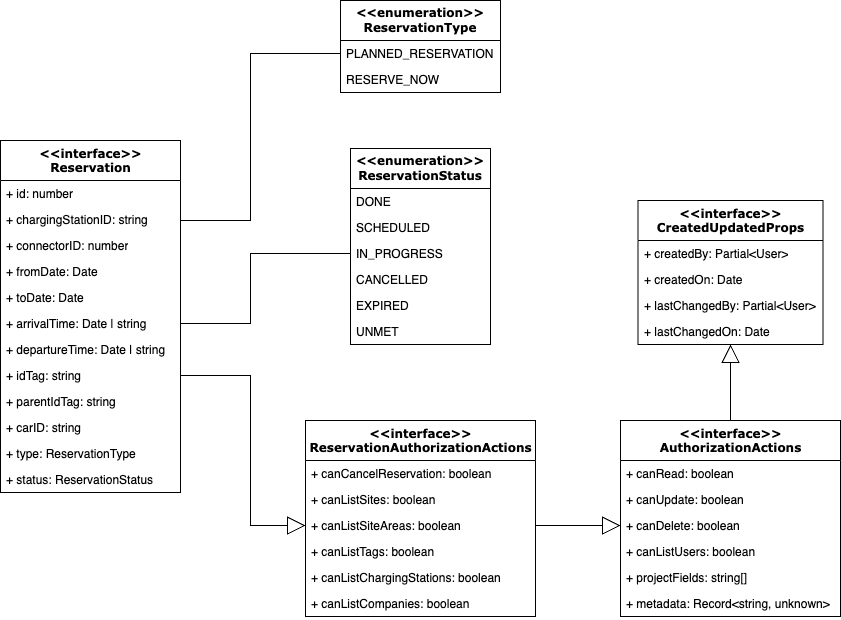
\includegraphics[scale=0.4]{resources/images/main/6_implementation/Reservation.png}
    \caption{Class diagram for the elaborated entity and its associated classes.}
    \label{fig:reservation-class-diagram}
\end{figure}

\noindent Regarding the proposed associations with the included interfaces, the resulting implementation is equivalent to the design entity relationships, shown in Figure \ref{fig:entity-relationship-diagram}, from the previous chapter. Thus, no further class diagram illustrating the quantity of each entity within the relationship is necessary in this section.
According to the \texttt{Reservation} interface as the foundation for further development, the application proposal is the next stage of this part of the thesis. 

\section{Reservation System}
\label{ch:Implementation:sec:Reservation System}

In order to take up the groundwork provided by the construction of the \texttt{Reservation} entity and the process design, the development of the reservation system according to the gathered work is next.
For a better understanding of the application serving as a baseline for the elaborated extension, the system itself is analyzed, by considering different views on the system and its modules.
As a result, different views out of the context of software architecture are used, to facilitate interested readers of this work to come up with an own implementation, utilizing the provided design approaches.

\subsection{Architectural Views}
\label{ch:Implementation:sec:Reservation System:ssec:System Architecture}

Starting with a high--level view of the existing system architecture, to identify the existing components and interfaces incorporated by the backend. 
For this reason, the module view of the backend system, shown below in Figure \ref{fig:module-view}, provides a detailed insight into the system itself, to discover the standards utilized and their associated functionalities, which are implemented as dedicated servers.
To present this highly abstract point of view, these modules are represented as functional units in terms of the decomposition style described by Clements~et al.~\cite[p.~67]{clements_documenting_2011}.
This architectural style is frequently used in order to divide the system into units of implementation that enable better structuring.
Regarding the assumptions of this work, the most significant modules and interfaces including the \acrshort{rest} server, the \textbf{WebSocket} interfaces, and the \acrshort{odata} interface, due to its growing importance in the business world and for the purpose of completeness.
In respect of the prefix used, each server responds to a different type of communication protocol to provide a specific set of features.
Enabling several clients to use the \acrshort{rest} protocol for communication purposes, the \texttt{REST Server} allows data exchange based on \acrshort{http} requests, facilitating the \acrshort{rest} principles, described in Subsection \ref{ch:Fundamentals:sec:Data Exchange:ssec:REST}. 
For this purpose, this server encloses the functionality of the subsequent servers, using so--called \acrshort{rest} resources to provide homogeneous entry points, that the clients could use to communicate with the servers behind it, without knowledge about each specific resource. 
In the case of the \textbf{WebSocket} interface, the backend system provides a reliable way to exchange data in real--time, using the \textbf{WebSocket} protocol mentioned in Subsection \ref{ch:Fundamentals:sec:Data Exchange:ssec:WebSocket}. 
Primarily, this interface is used to communicate with the managed charging infrastructure, including directly accessing the \texttt{\acrshort{ocpp} Server} for the administration of \acrshortpl{cs}.
The \texttt{\acrshort{odata} Server}, with the inclusion of the \textbf{\acrshort{odata} REST Interface}, allows \acrshort{odata} clients to access the backend functionalities. 
By enhancing the capabilities of the standard \acrshort{rest} protocol through publishing a public description of the offered services, in the form of a description document similar to the \acrshort{soap} \acrshort{wsdl}, it provides an alternative for utilizing the services in more advanced scenarios.

\begin{figure}[h]
    \centering
    \includegraphics[scale=0.4]{resources/images/main/6_implementation/DeploymentView.png}
    \caption{Overview of the various functional components within the existing project.}
    \label{fig:module-view}
\end{figure}

\noindent As indicated by Figure \ref{fig:module-view}, and due to the reliance on the targeted client applications, which primarily use \acrshort{rest} based communication, the main development work is located within the \texttt{REST server}. 
Besides its role of mapping functionality to the outside world, the corollary of integrating the reservation system inside this server is considered trivial.
For a deeper understanding of the internal structure of this server, and to reduce the architectural height to identify the relevant components and packages, for the required changes to implement the extension accordingly, the following sub--parts drill down to provide a more detailed view.

\subsubsection{Packages}
\label{ch:Implementation:sec:Reservation System:ssec:Architectural Views:sssec:Packages}

After the choice of the \texttt{REST server} as the location for the functionalities, the introduced architectural style of decomposition, allows for the arbitrary adjustment of the perspective into which a system and its modules could be further subdivided.
As part of Figure \ref{fig:package-view}, the utilized extraction process of relevant modules into packages that structure the application is displayed. This view not only shows the logical structure of the project but also allows developers to group together functionality or logical units with a high degree of cohesion in a particular location.
As introduced in the previous section with reference to the class diagram \ref{fig:reservation-class-diagram} for the reservation type, the entity, also known as a type, can be located within the \texttt{types} package. 
The \texttt{requests}, which represent pre--defined request bodies for the request \texttt{validator} instances, sanitize incoming payloads before processing. Following this naming convention, applicable to all types of implementations in the application structure, the corresponding packages could be easily identified.
So the appropriate implementations for \texttt{router} and \texttt{service}, to provide the \acrshort{rest} resources, as well as the \texttt{storage} classes for database access, can be readily determined. 
Also worth mentioning is the mapping of permissions for the existing roles within the \texttt{authorisation} package, the addition of \texttt{notification} types to notify the user, and the integration of new \texttt{tasks} to provide scheduled background jobs for autonomous reservation processing.
However, all of these artifacts and their associated changes are addressed in the following sections and are presented solely for awareness of their existence.

\begin{figure}[h]
    \centering
    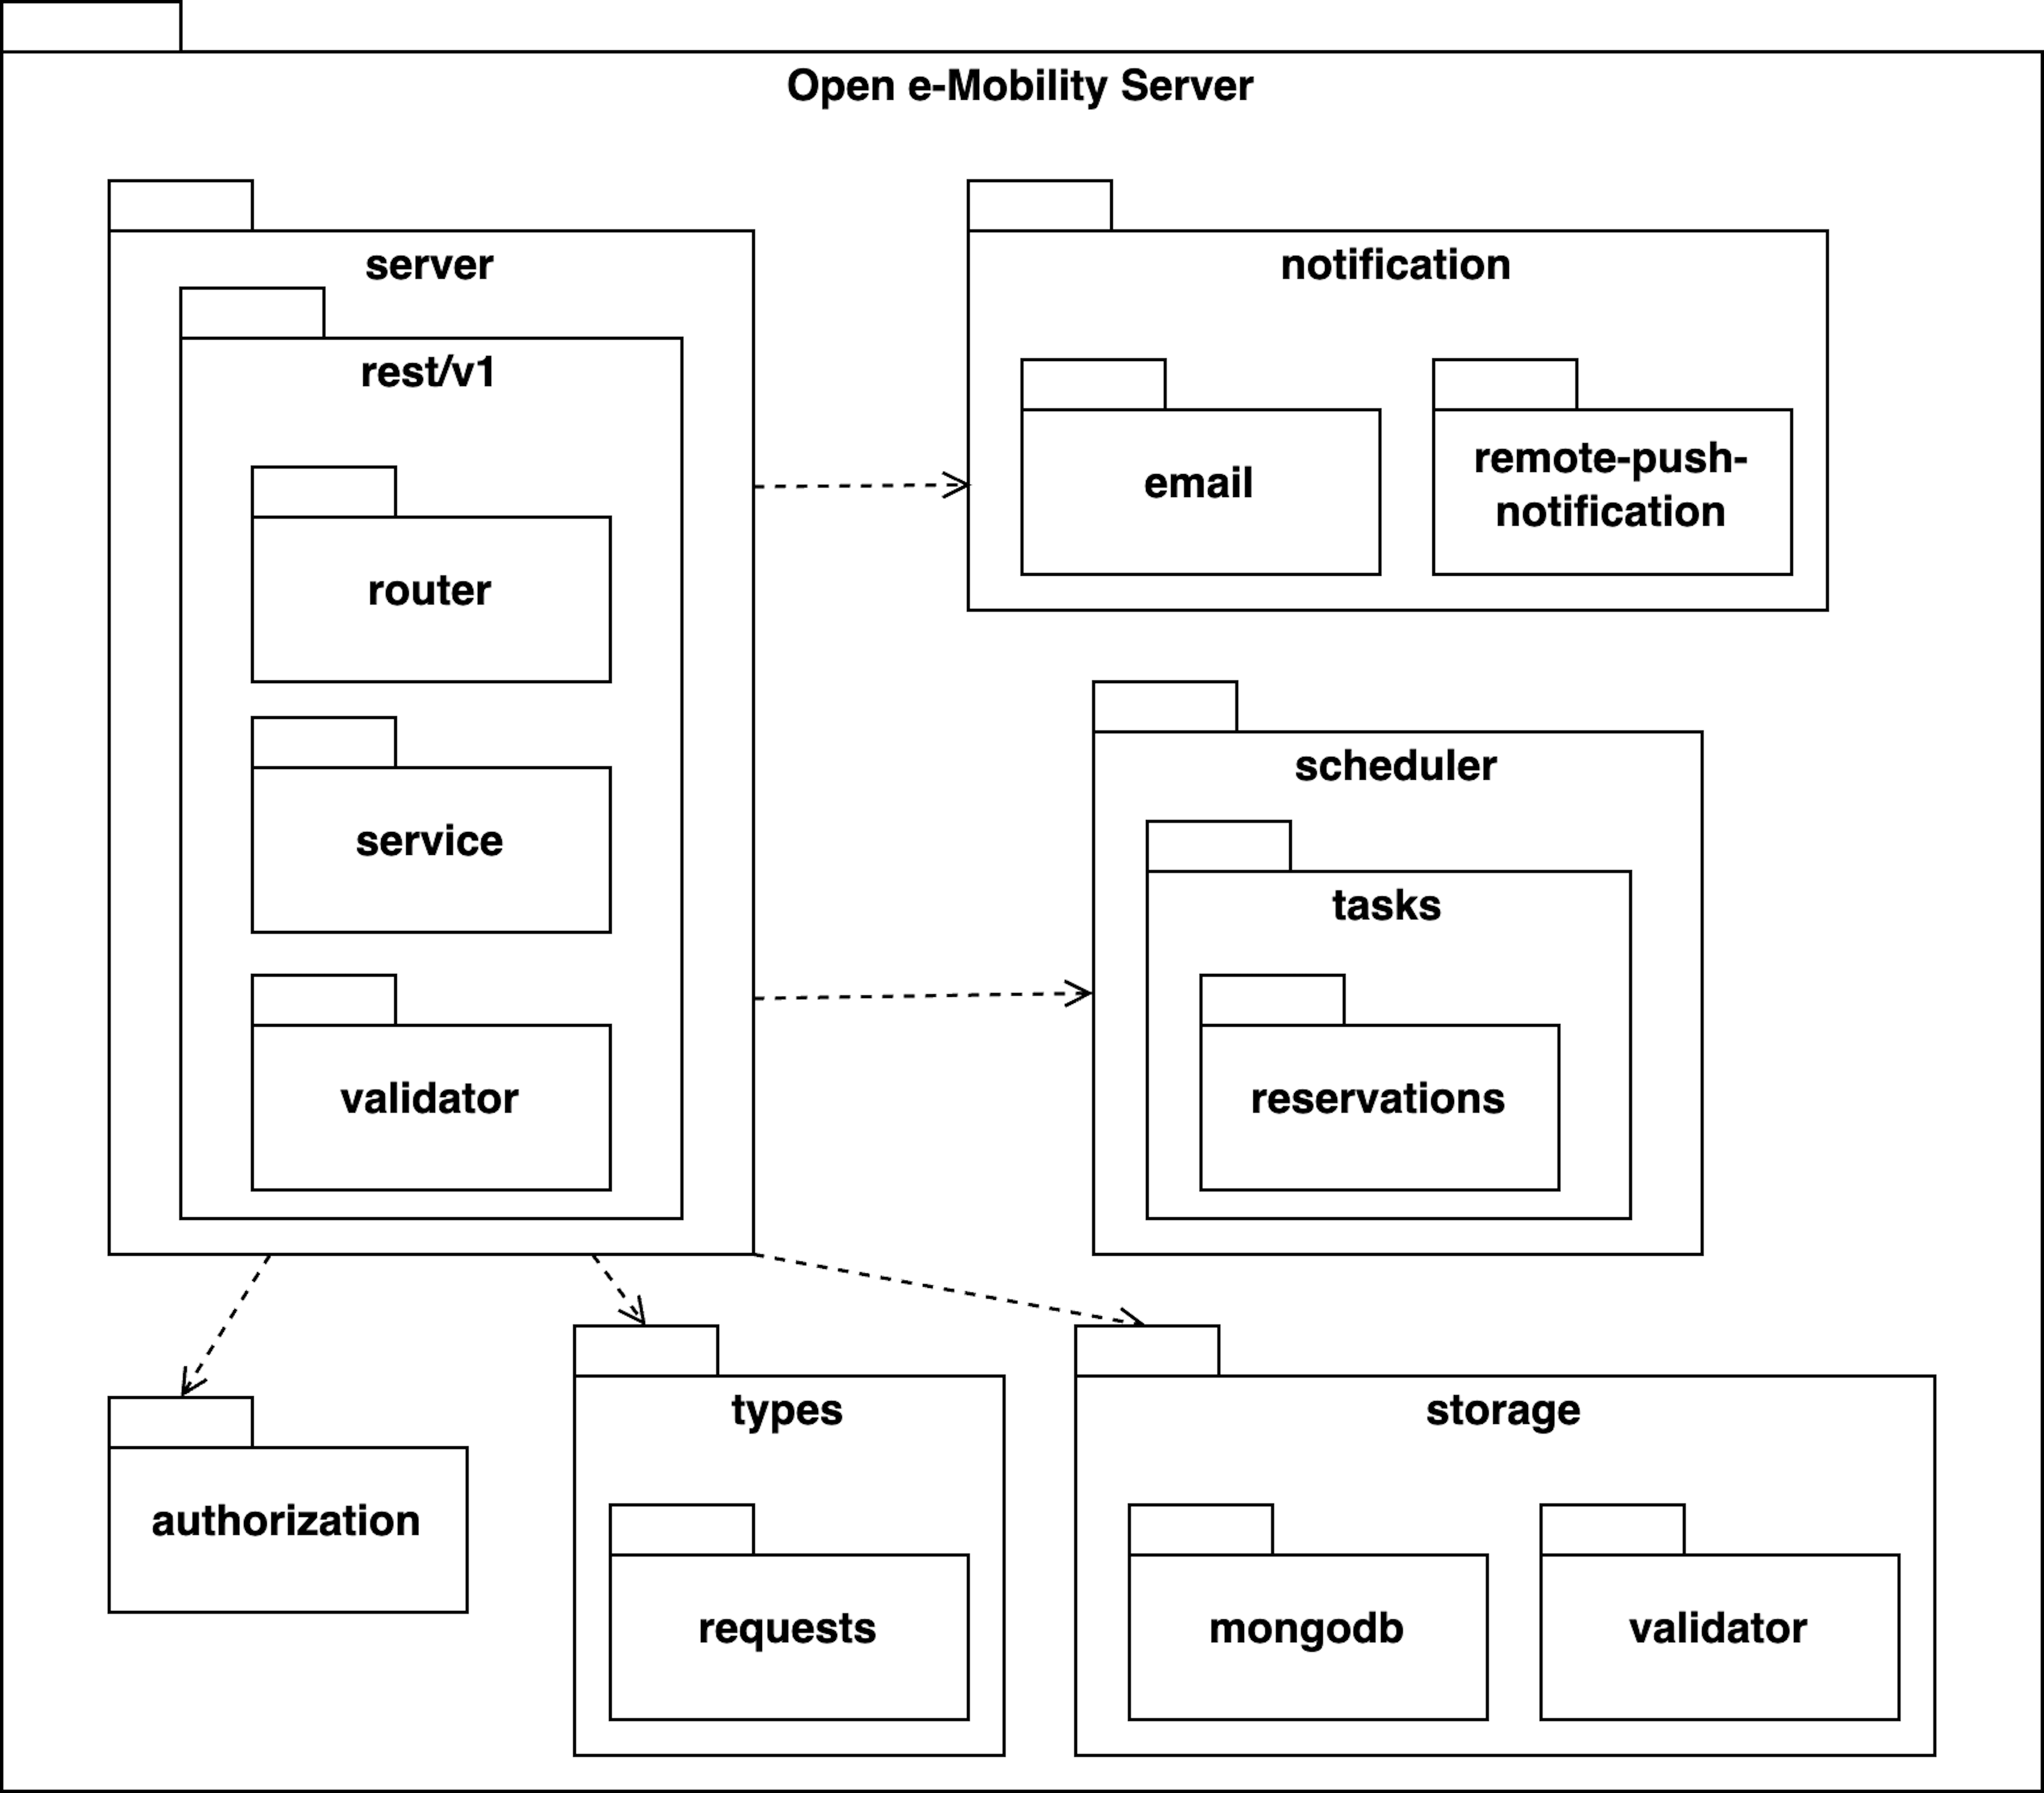
\includegraphics[scale=0.4]{resources/images/main/6_implementation/PackageDiagram.png}
    \caption{Overview of the extended packages within the targeted section of the backend project.}
    \label{fig:package-view}
\end{figure}

\noindent With the structure of the service and the location of the adaptations in mind, the next step is to introduce the components and their associated connectors. 
Architecturally, the 'component--and--connector views (C\&C)'~\cite[p.~136]{clements_documenting_2011} are used to show the inner workings of the system and the interaction between the individual components. 
Concerning the follow--up implementation, this aspect could be used for orientation and guidance in the project and provide a starting point for further development tasks, to locate the changes introduced by this work.

\subsubsection{Components}
\label{ch:Implementation:sec:Reservation System:ssec:Architectural Views:sssec:Components}

Before elaborating on the behavioral interaction between the components, all the implemented aspects have to be mapped in the context of the designed system. Thus, Figure \ref{fig:component-view} provides an overview of the added components and their integration with the already existing ones.
In line with the C\&C view, the connectors indicate the available and required functionalities and establish the appropriate connections between the corresponding components, resulting in the reservation system as part of the existing service landscape.
For the purpose of abstraction between the existing implementations and the extension, this work treats the \texttt{Reservation System} as an independent subsystem that requires only a restricted number of dependencies to other areas of the application.
Considering only the information required from other application domains, the portability as a self--contained system to other scenarios should be guaranteed.

\begin{figure}[h]
    \centering
    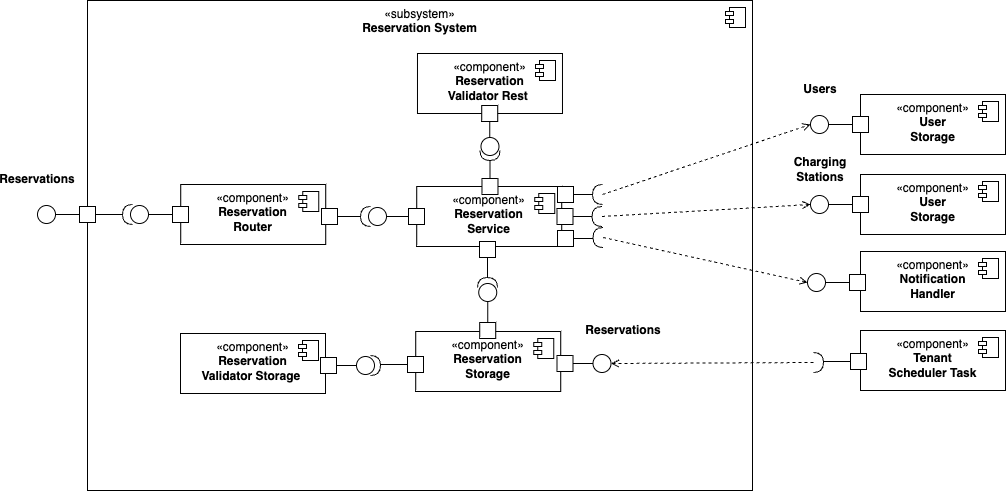
\includegraphics[scale=0.4]{resources/images/main/6_implementation/ReservationComponents.png}
    \caption{Overview of the individual components inside the extended web service.}
    \label{fig:component-view}
\end{figure}

\noindent Taking the design principles of the initial developers and the previously mentioned package structure into account, the \texttt{Reservation System} must contain several classes necessary for the \acrshort{rest}ful web service implementation.
This includes the use of a \texttt{Reservation Router} that manages incoming requests of client applications and allocates them to the relevant methods offered by the \texttt{Reservation Service}, determined by the requested resource and the parameters in the \acrshort{url}.
In the majority of cases, data is requested, which is provided by the \texttt{Reservation Storage}, encapsulating the access to the database and maintaining the lifetime of the corresponding connection.
To verify the entities arriving with the \acrshort{http} request bodies that are to be persisted in the database, the \texttt{Reservation~Validator~Rest} after receiving the requests and the \texttt{Reservation~Validator~Storage} before further processing in the database, form the first layer of validation, to prevent malformed input.
Finally, the \texttt{Notification~Handler} and the \texttt{Tenant~Scheduler~Task} represent pre--existing components utilized by the \texttt{Reservation System} for supportive purposes and are not an explicit part of the system itself.
According to its name, the \texttt{Notification Handler} is responsible for dispatching notifications to the relevant user in certain cases and the \texttt{Tenant Scheduler Task} coordinates background operations. 
By guaranteeing an entryway for external components and systems that require reservation capabilities, the \texttt{Reservation} interface, which points outside the system, allows access to the implemented functionalities inside.
On the basis of the elaborated components and their location within the architectural construct of the application, the next subsection continues to illustrate the relevant information flow and interaction to achieve the capabilities in relation to the design work.

\subsection{Management Capabilities}
\label{ch:Implementation:sec:Reservation System:ssec:Management Capabilities}

Combining the designed processes and the aforementioned architectural views, the next parts describe the actual functionality implemented within the system, while keeping the implemented components in mind.
Beginning with the management capabilities for the respective entities, which include creation, update, deletion, and cancellation offered as the basic operations offered by this functional module. This also incorporates the administrative capability to enable the reservation extension. 
In order to gain insight into the implementation of the backend logic in the frontend parts, as well as the comparison with the previously designed mockups, this theoretical perspective is complemented by the final implementation in the frontend applications of the system.

\subsubsection{Create Reservation}
\label{ch:Implementation:sec:Reservation System:ssec:Management Capabilities:sssec:Create Reservation}

Beginning with the implementation of the \textbf{Create Reservation} functionality shown in Figure \ref{fig:create-reservation-seqflow} and executed every time receiving a request for creating a reservation from an actual user at the \texttt{ReservationRouter}. 
Delegated to the \texttt{ReservationService} by calling the \texttt{handleReservationCreate} method, the \texttt{ReservationValidatorRest} immediately validates the provided input and stops the execution and the further processing of the entity by detection of malformed or erroneous properties.
In case of a successful validation and the non--existence of a record with the same \acrshort{id}, the system checks for collisions with other bookings in the selected time range to prevent overbooking of a \acrshort{cs}.
After fulfilling all the required conditions for making a reservation, the selected \acrshort{cs} is contacted in case of a \textit{ReserveNow} reservation or a scheduled booking with an upcoming timeslot, and the entity is persisted through the \texttt{ReservationStorage}, after a final validation by the \texttt{ReservationValidatorStorage}.
Considering the scenario, if a record with the same \acrshort{id} exists, this design permits the existing reservation to be updated by conformity with the deposited \acrshort{rfid} tags as well. A mismatch otherwise results in the execution being aborted to prevent another user without the required privileges from adjusting the reservation.
Finally, a confirmation notification of the successfully created arrangement is sent to the concerned user.

\begin{figure}[h]
    \centering
    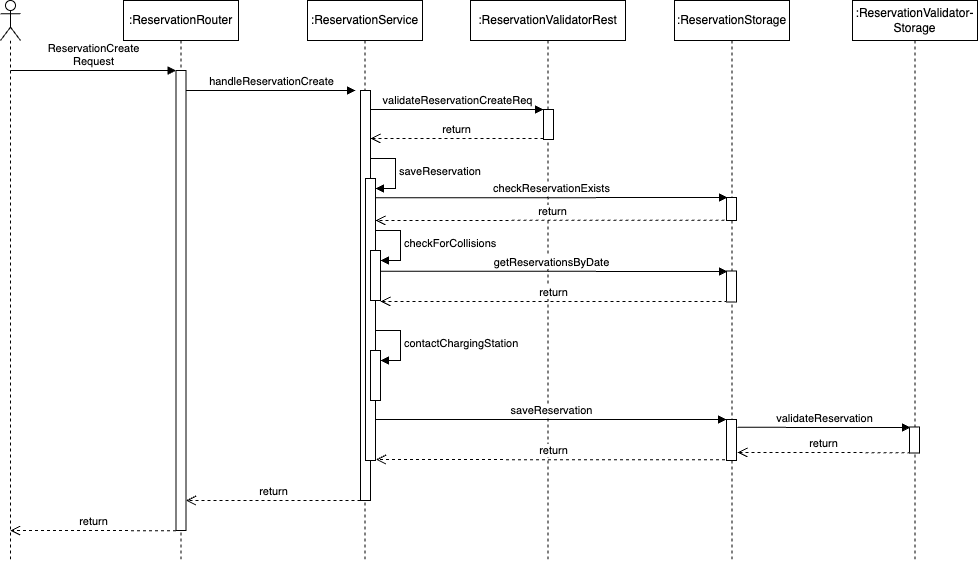
\includegraphics[scale=0.4]{resources/images/main/6_implementation/processes/ReservationCreate.png}
    \caption{Component interaction for fulfilling the process flow of creating a reservation in reference to the proposed design.}
    \label{fig:create-reservation-seqflow}
\end{figure}

\newpage

\noindent With the required booking properties in mind, the corresponding input screens of the mobile and web applications resulted in the subsequent layout shown in Figure \ref{fig:impl-create-reservation}. 
As well as mapping the relevant properties to the input fields on the user interfaces, the existing layout plays a crucial role in the proposed appearance of the result.
For supporting both types of reservations elaborated in this work, a selection toggle is implemented, which appears when the proposed extension is enabled for the respective tenant and automatically adjusts the displayed options on behalf.
In combination with an integrated validation of the input fields, the approach to provide one central interface as an entry point for creating the reservation should allow for maximum convenience for the user.
Another aspect to mention is, that the selection of a \texttt{Parent \acrshort{id} Tag}, representing a superior \acrshort{rfid} tag for a group of subordinate tags, is not considered in this particular implementation. 
This simplifies the handling of the data model and enables a one--to--one relationship between the user and the reservation.
Although the input option is absent in the frontend, the associated property indeed exists in the underlying entity.

\begin{figure}[h]
    \centering
    \begin{subfigure}[c]{0.6\textwidth}
        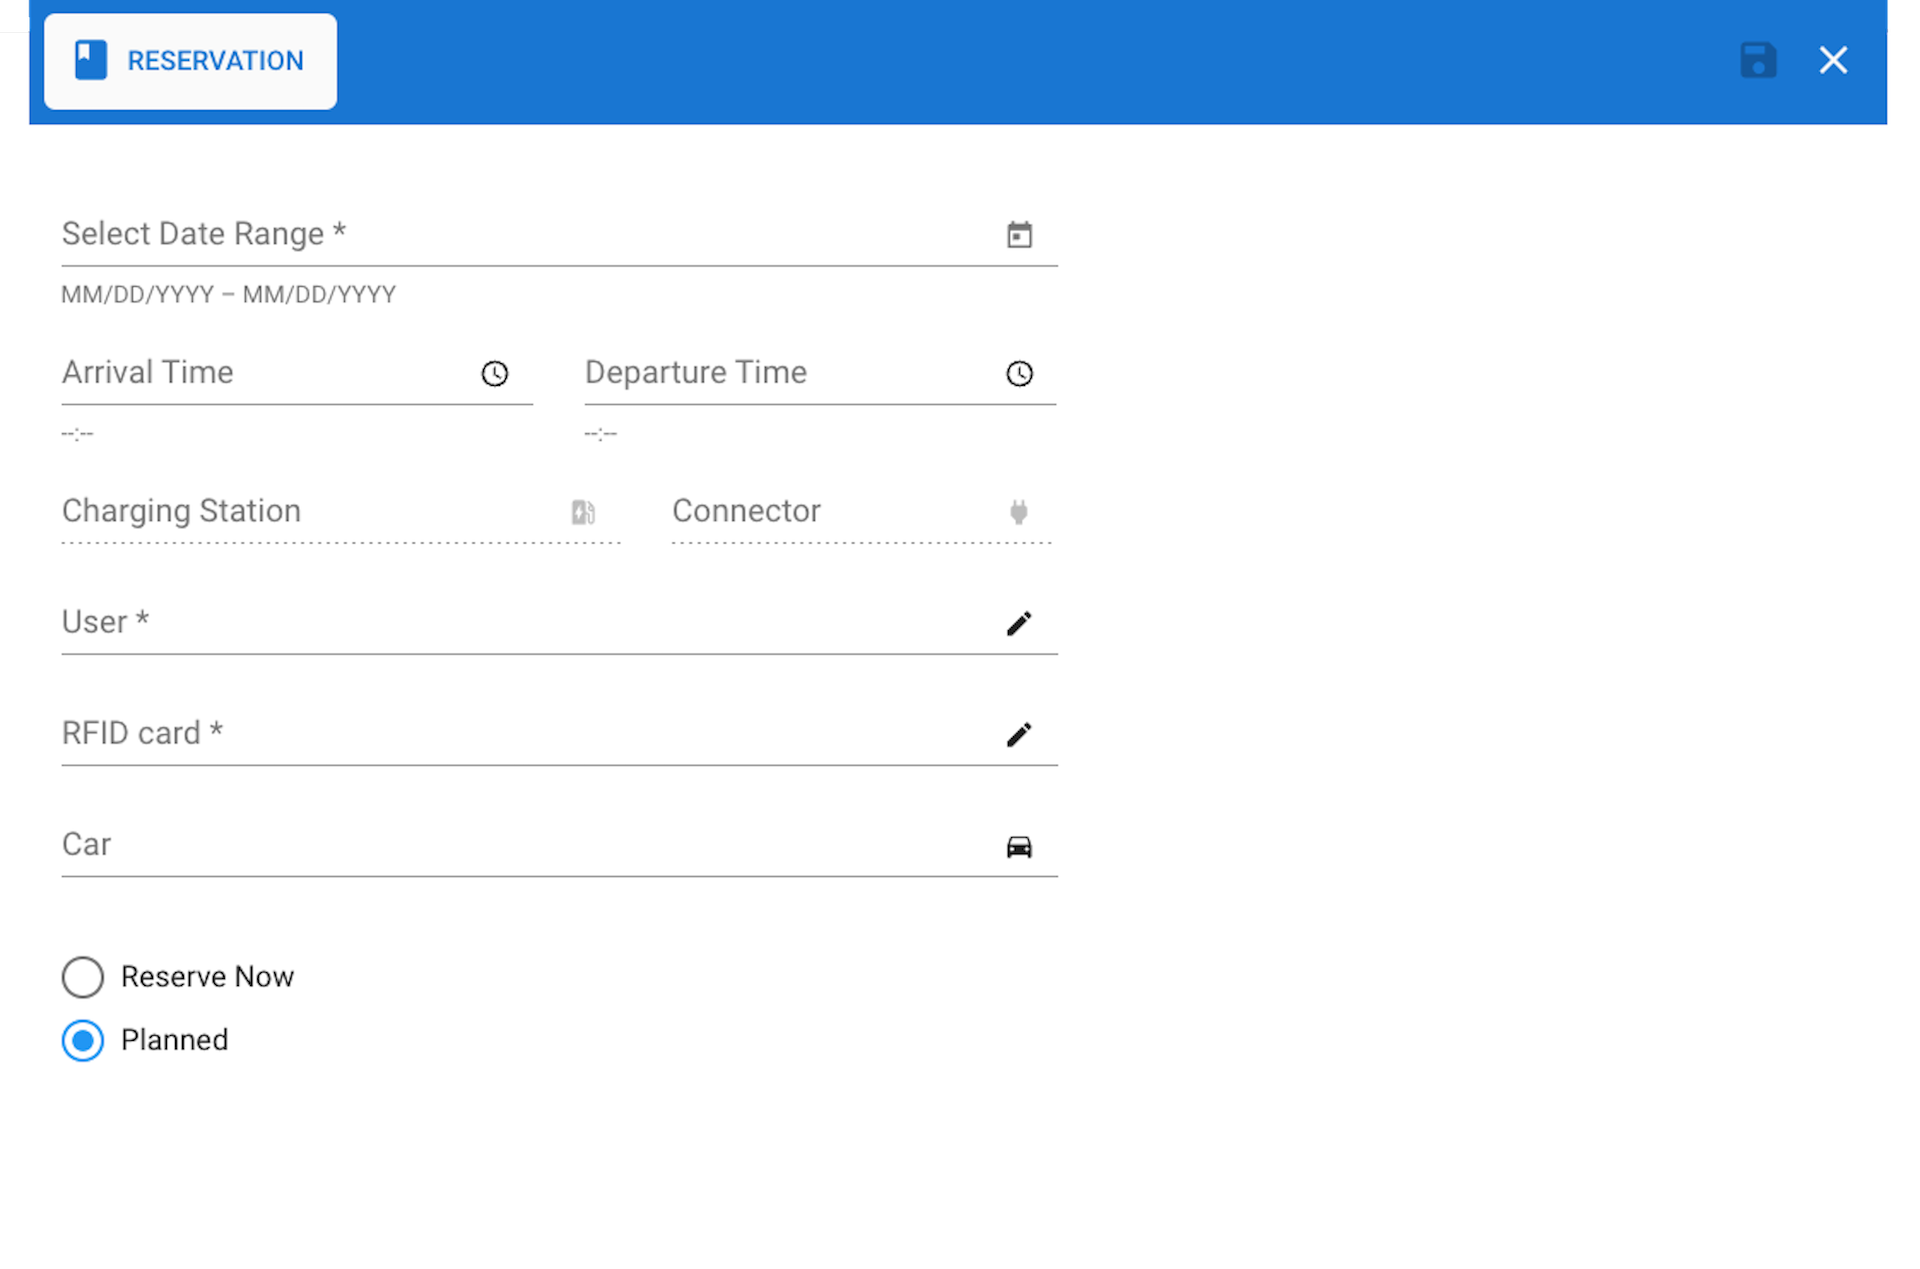
\includegraphics[width=\textwidth]{resources/images/main/6_implementation/screens/create_reservation/web/Create_Reservation.png}
        \captionsetup{skip=30pt}
        \caption{Create a reservation in the web application.}
        \label{fig:web-create-reservation-impl}
    \end{subfigure}
    \hfill
    \begin{subfigure}[c]{0.3\textwidth}
        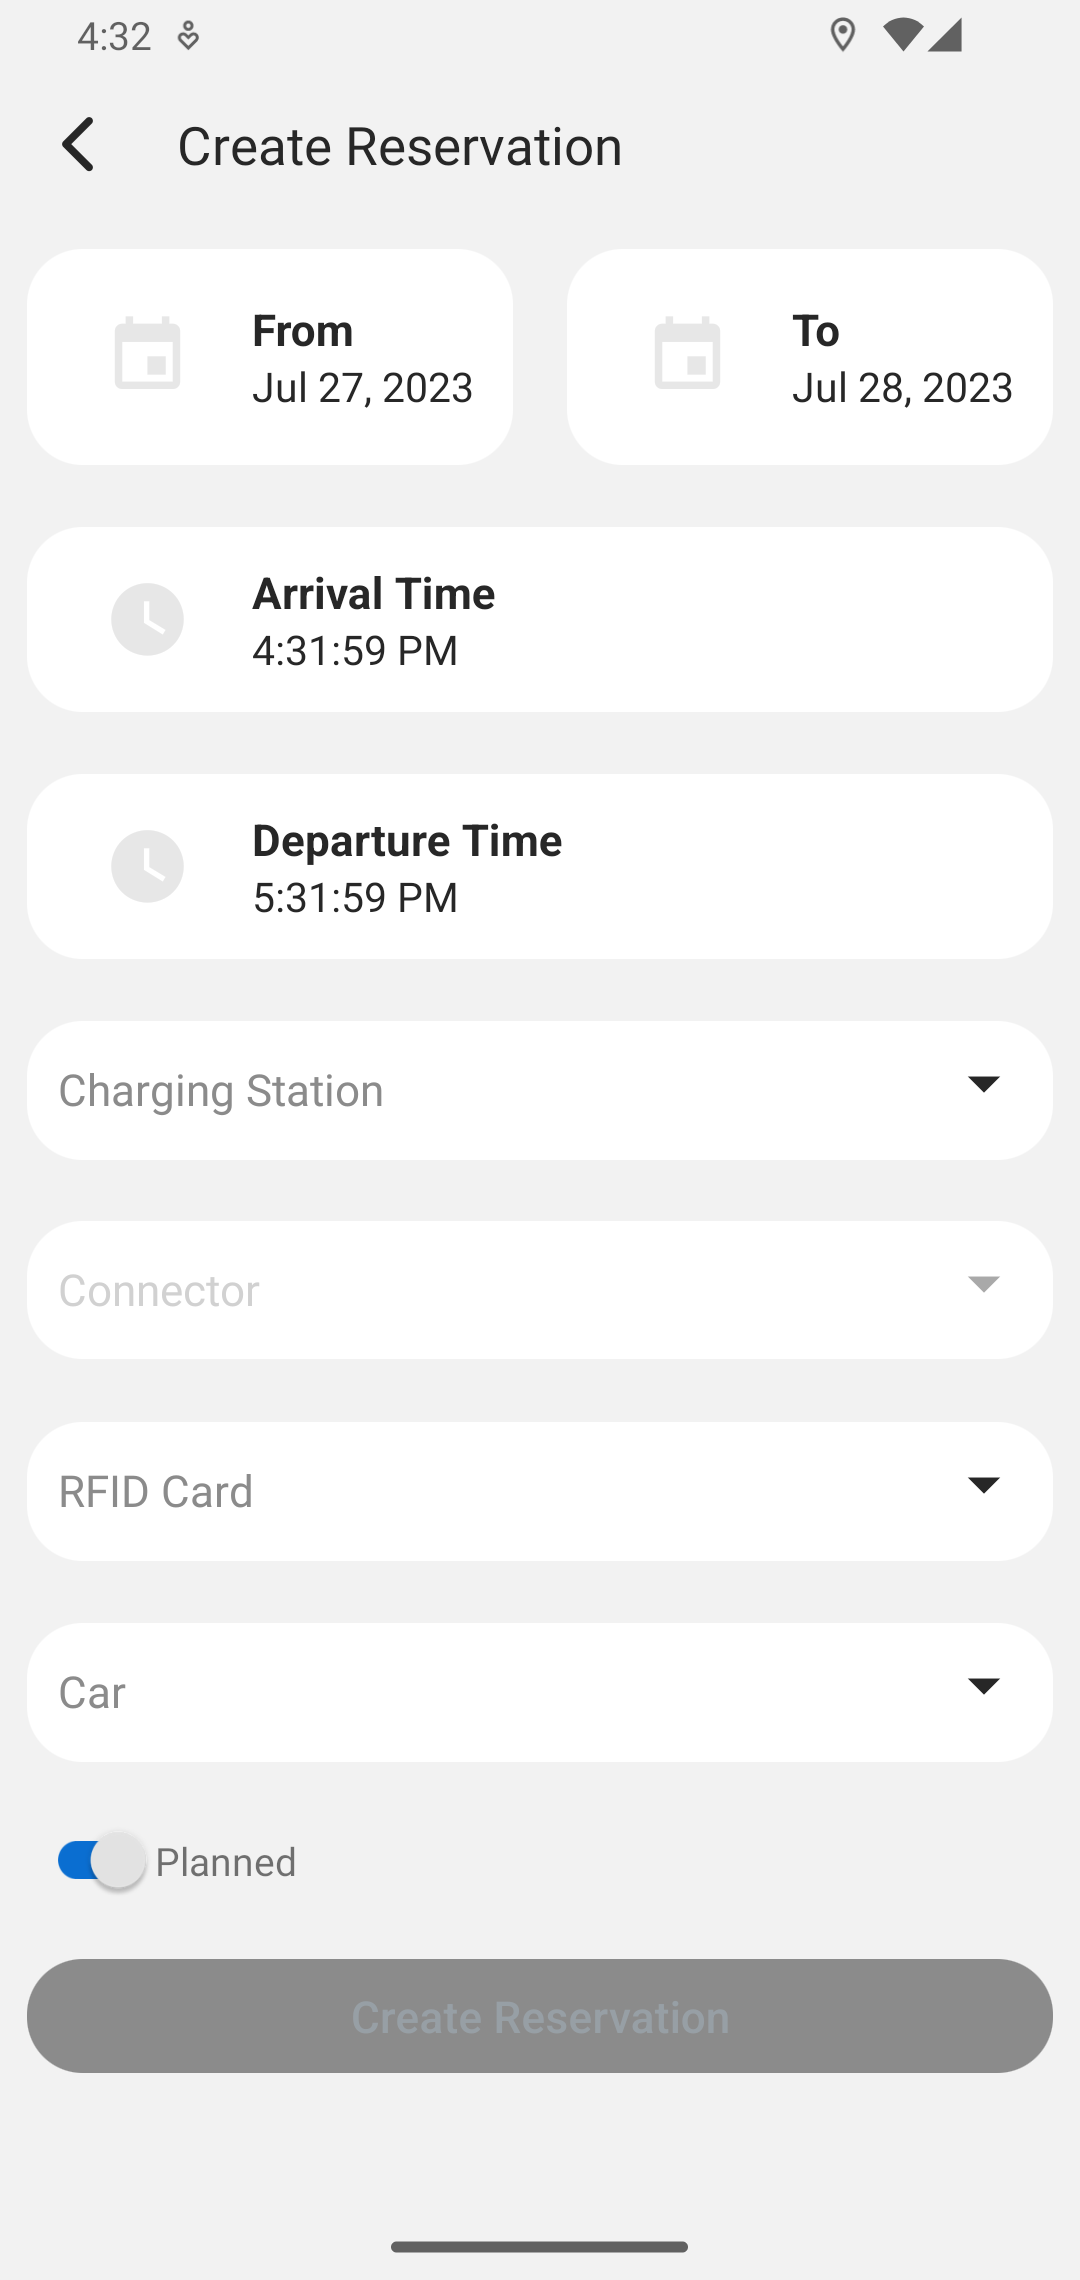
\includegraphics[width=\textwidth,height=1.6\textwidth,keepaspectratio]{resources/images/main/6_implementation/screens/create_reservation/mobile/Create_Reservation.png}
        \caption{Create a reservation in the mobile application.}
        \label{fig:mobile-create-reservation-impl}
    \end{subfigure}
    \caption{Implementation of the user interfaces of the mobile and web application relating to the creation of reservations.}
    \label{fig:impl-create-reservation}
\end{figure}

\noindent Delivering this functionality using the \acrshort{rest} methodology and the appropriate resource, the \textbf{Create Reservation} process could be called on behalf of the following endpoint listed in Table \ref{tab:create-reservation-rest}.

\begingroup
\setlength{\tabcolsep}{10pt} % Default value: 6pt
\renewcommand{\arraystretch}{1.5} % Default value: 1
\begin{table}[h]
\centering
\caption{\acrshort{rest} endpoint for reservation creation.}
    \begin{tabular}{l|c}
    Resource Identifier & HTTP Method \\ \hline
    \texttt{/reservations/} & \texttt{POST} \\    
    \end{tabular}
\label{tab:create-reservation-rest}
\end{table}
\endgroup

\newpage

\subsubsection{Update Reservation}
\label{ch:Implementation:sec:Reservation System:ssec:Management Capabilities:sssec:Update Reservation}

Despite the similarities to the previously mentioned creation process in relation to the details covered, the \textbf{Update Reservation}, pictured in Figure \ref{fig:update-reservation-seqflow}, typically expects that the arrangement the user wants to update already exists.
In conformity with its logical twin, the user request passes through \texttt{ReservationRouter} and is forwarded by the \texttt{handleReservationUpdate} method to the \texttt{ReservationService}, which implements the required update logic.
Then, \texttt{ReservationValidatorRest} performs the initial input validation, before querying the reservation associated with the provided \acrshort{id} through \\ \texttt{ReservationStorage}.
Because of the aforementioned overlaps between the creation and updating process, no further description of the other steps undertaken is given in order to avoid repetition, which results from the fact that the system updates reservations in a manner, comparable to the \acrshort{cs} outlined in the \acrshort{ocpp} standard.
As indicated there, an existing entity with the same \acrshort{id} is replaced by any incoming \textit{ReserveNow} request with the same \acrshort{id}.  
Such a flawed design could allow the cancellation of reservations made by other users, who have the same \acrshort{id} as the existing object at the station, which should be prevented. So, the proposed system approach implements a check for this uncommon but potential scenario.
Relating to future work, this behavior should be observed, as it is still included in the latest \acrshort{ocpp} version 2.0 specification.
In order to handle alterations to the \acrshort{cs} or connector, the updating procedure guarantees the revocation of the booking at the previous station and gets in contact with the new station accordingly.

\newpage

\begin{figure}[h]
    \centering
    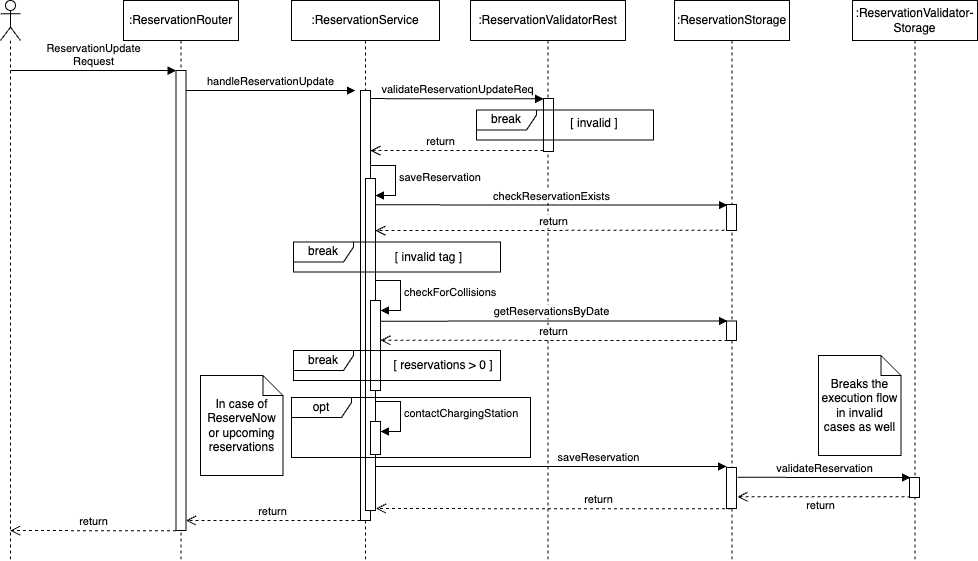
\includegraphics[scale=0.4]{resources/images/main/6_implementation/processes/ReservationUpdate.png}
    \caption{Component interaction for updating a reservation considering the proposed design draft.}
    \label{fig:update-reservation-seqflow}
\end{figure}

\noindent Because of the parallels in the underlying process, the interfaces for facilitating the update of an entity, include the same input choices as the interface designed for creation.
The sole variation within the browser application is the ability to cancel the booking within the update mask using the auxiliary \textbf{Cancel Reservation} button shown in \ref{fig:web-update-reservation-impl}. 
This feature has not been integrated into the mobile app for reasons of limited screen space and to minimize the amount of information displayed to avoid cluttered screens.

\begin{figure}[h]
    \centering
     \begin{subfigure}[c]{0.6\textwidth}
         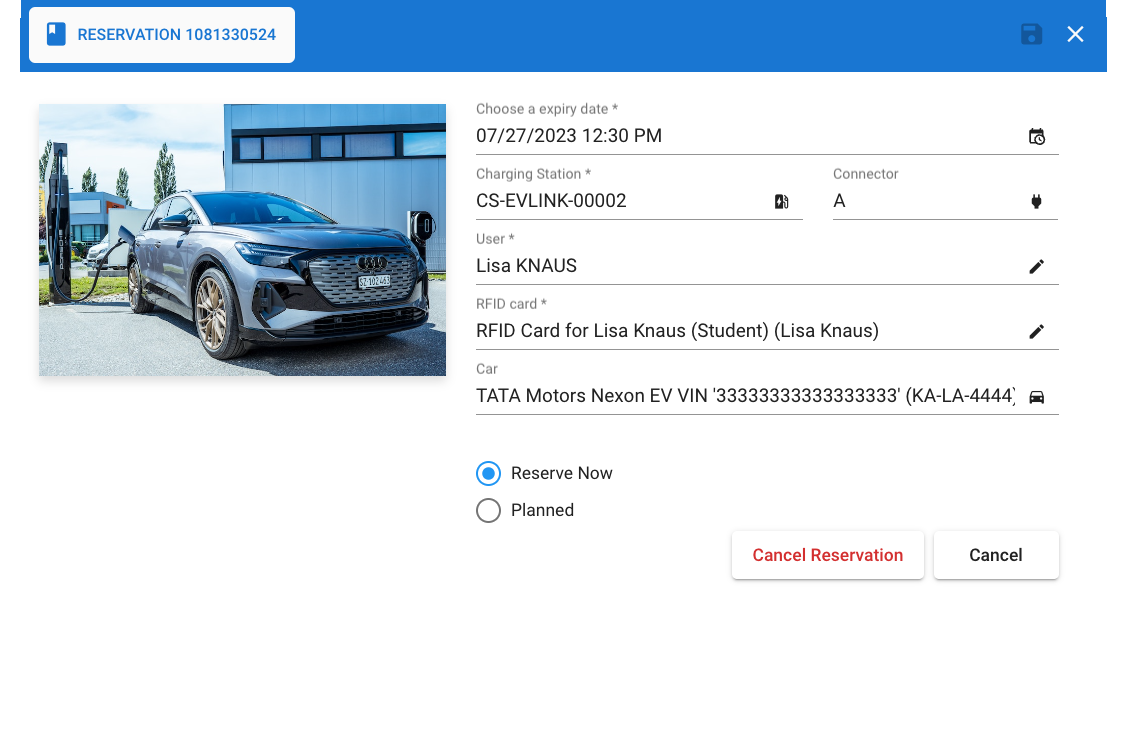
\includegraphics[width=\textwidth]{resources/images/main/6_implementation/screens/update_reservation/web/Update_Reservation.png}
         \captionsetup{skip=33pt}
         \caption{Update a reservation in the web application.}
         \label{fig:web-update-reservation-impl}
    \end{subfigure}
     \hfill
     \begin{subfigure}[c]{0.3\textwidth}
         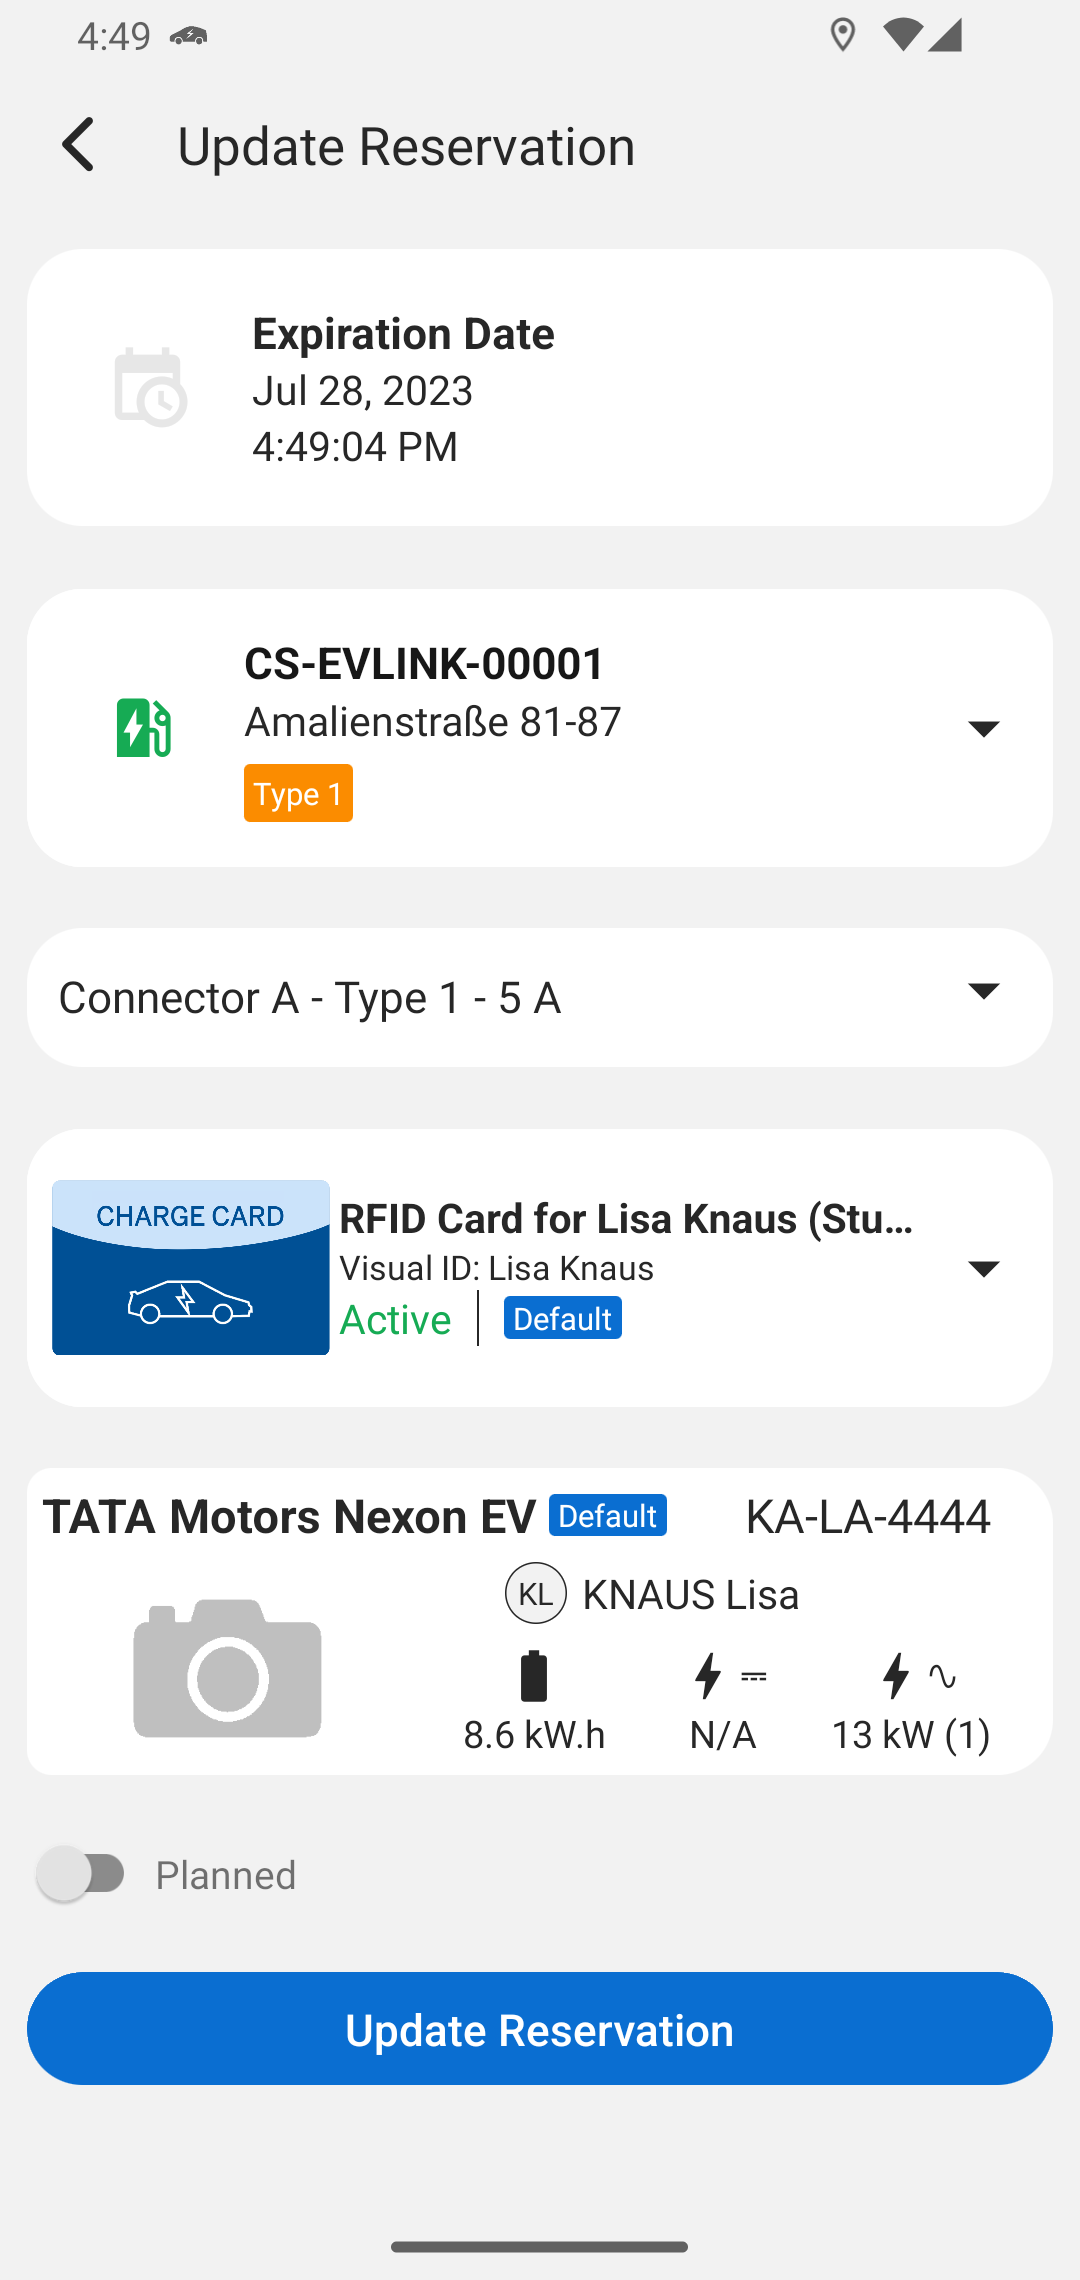
\includegraphics[width=\textwidth,height=1.6\textwidth,keepaspectratio]{resources/images/main/6_implementation/screens/update_reservation/mobile/Update_Reservation.png}
         \caption{Update a reservation in the mobile application.}
         \label{fig:mobile-update-reservation-impl}
    \end{subfigure}
    \caption{Implementation of the user interfaces of the mobile and web applications to update a reservation.}
    \label{fig:impl-update-reservation}
\end{figure}

\noindent For the interaction with the relevant client apps, the \textbf{Update Reservation} process could be called on behalf of the following \acrshort{rest} interfaces listed in Table \ref{tab:update-reservation-rest}.

\begingroup
\setlength{\tabcolsep}{10pt} % Default value: 6pt
\renewcommand{\arraystretch}{1.5} % Default value: 1
\begin{table}[h]
\centering
\caption{\acrshort{url} with path parameter for initiating an update using the respective \acrshort{rest} resource.}
    \begin{tabular}{l|c}
    Resource Identifier & HTTP Method \\ \hline
    \texttt{/reservations/\{id\}} & \texttt{PUT}
    \end{tabular}
\label{tab:update-reservation-rest}
\end{table}
\endgroup

\newpage

\subsubsection{Cancel Reservation}
\label{ch:Implementation:sec:Reservation System:ssec:Management Capabilities:sssec:Cancel Reservation}

Derived from the \textbf{Update Reservation} procedure described in \ref{ch:Implementation:sec:Reservation System:ssec:Management Capabilities:sssec:Update Reservation}, the \textbf{Cancel Reservation} operation enables the requestor, the revocation of a scheduled or already ongoing arrangement as illustrated in Figure \ref{fig:cancel-reservation-seqflow}.
Like its predecessors, the initiation of the downstream logic in the \texttt{ReservationService} undergoes the initial validation checks after request delegation by the \texttt{ReservationRouter}.
This ensures, that the incoming inquiry aligns according to the defined criteria within the solution and mitigates unintentional behavior, resulting from malformed user input.
By not ending the process prematurely due to erroneous data, the actual cancellation functionality within the service method \texttt{cancelReservation} is initiated.
Starting with the retrieval of the record from the database using the provided \acrshort{id}, the validation of the life cycle transition of the current status, as discussed in \ref{ch:Design:sec:Reservation:ssec:Reservation Status}, follows.
This ensures that only those objects that are suitable for cancellation, can be cancelled by the user and the system, otherwise, the process is terminated.
If the scheduled arrival time is already reached, the corresponding \acrshort{cs} is contacted, resulting in an immediate cancellation at that station.
After updating the status to \texttt{Cancelled}, in the case of a cancelled reservation, and successfully validating it once more, the entity is saved to the database again. The act of withdrawing a booking concludes with an outgoing cancellation notification from the \texttt{NotificationHandler} to the appropriate system user.

\newpage

\begin{figure}[h]
    \centering
    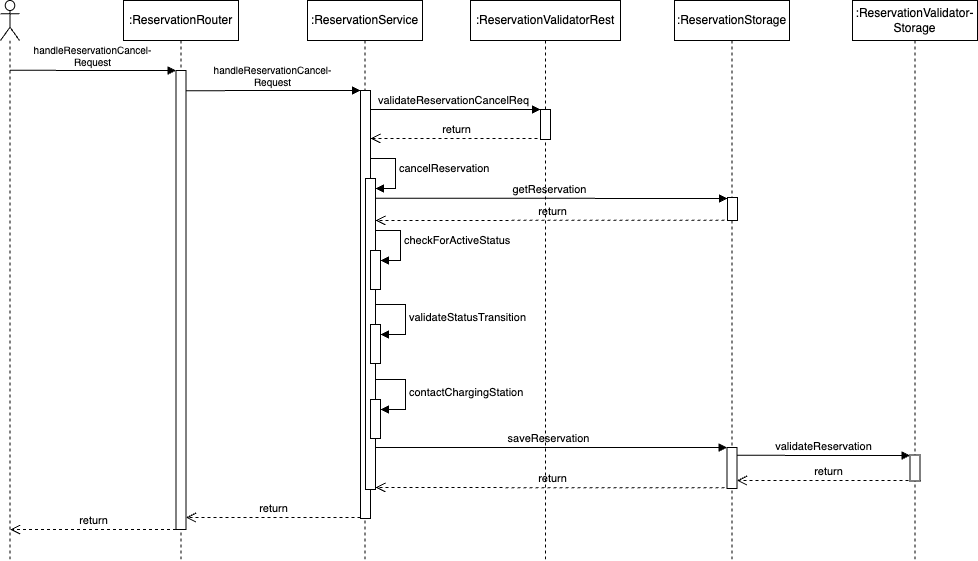
\includegraphics[scale=0.4]{resources/images/main/6_implementation/processes/ReservationCancel.png}
    \caption{The engagement of the different components during the cancellation of a reservation as proposed in the design.}
    \label{fig:cancel-reservation-seqflow}
\end{figure}

\noindent In terms of its impact on the entity and its existence within the application life cycle, the deletion of a reservation is more invasive than cancellation, which represents a practically identical atomic function, that could be realized through one single button. 
This thought led to the conclusion that such a button should be placed on each booking item on the relevant screen. Accordingly, these buttons should indicate that pressing them results in the associated cancellation of that particular booking.
In contrast to the mobile app, the webpage version permits the possibility of withdrawing already within the list overview. Enabling the user to interact more quickly with the appropriate entities, based on their current role and the assigned sites.
An example of the list view with the quick action buttons displayed at the list item level is shown in Figure \ref{fig:web-cancel-reservation-impl}, including an indicator pointing to the relevant button.

\begin{figure}[h]
    \centering
    \begin{subfigure}[c]{0.6\textwidth}
        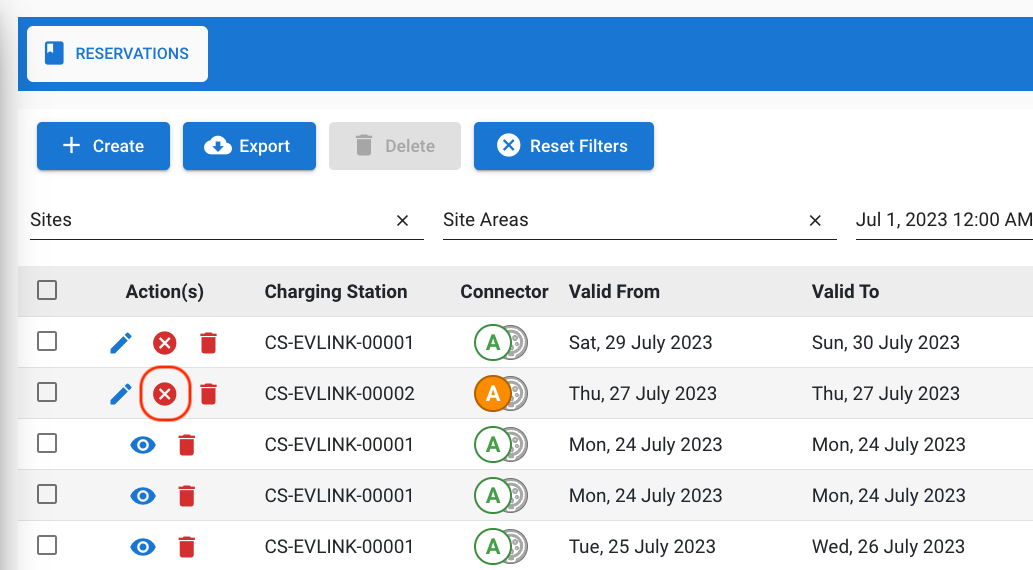
\includegraphics[width=\textwidth]{resources/images/main/6_implementation/screens/cancel_reservation/web/Cancel_Reservation.png}
        \captionsetup{skip=43pt}
        \caption{Cancel a reservation in the browser version of the app by using the \faIcon[solid]{times-circle} icon.}
        \label{fig:web-cancel-reservation-impl}
    \end{subfigure}
    \hfill
    \begin{subfigure}[c]{0.3\textwidth}
        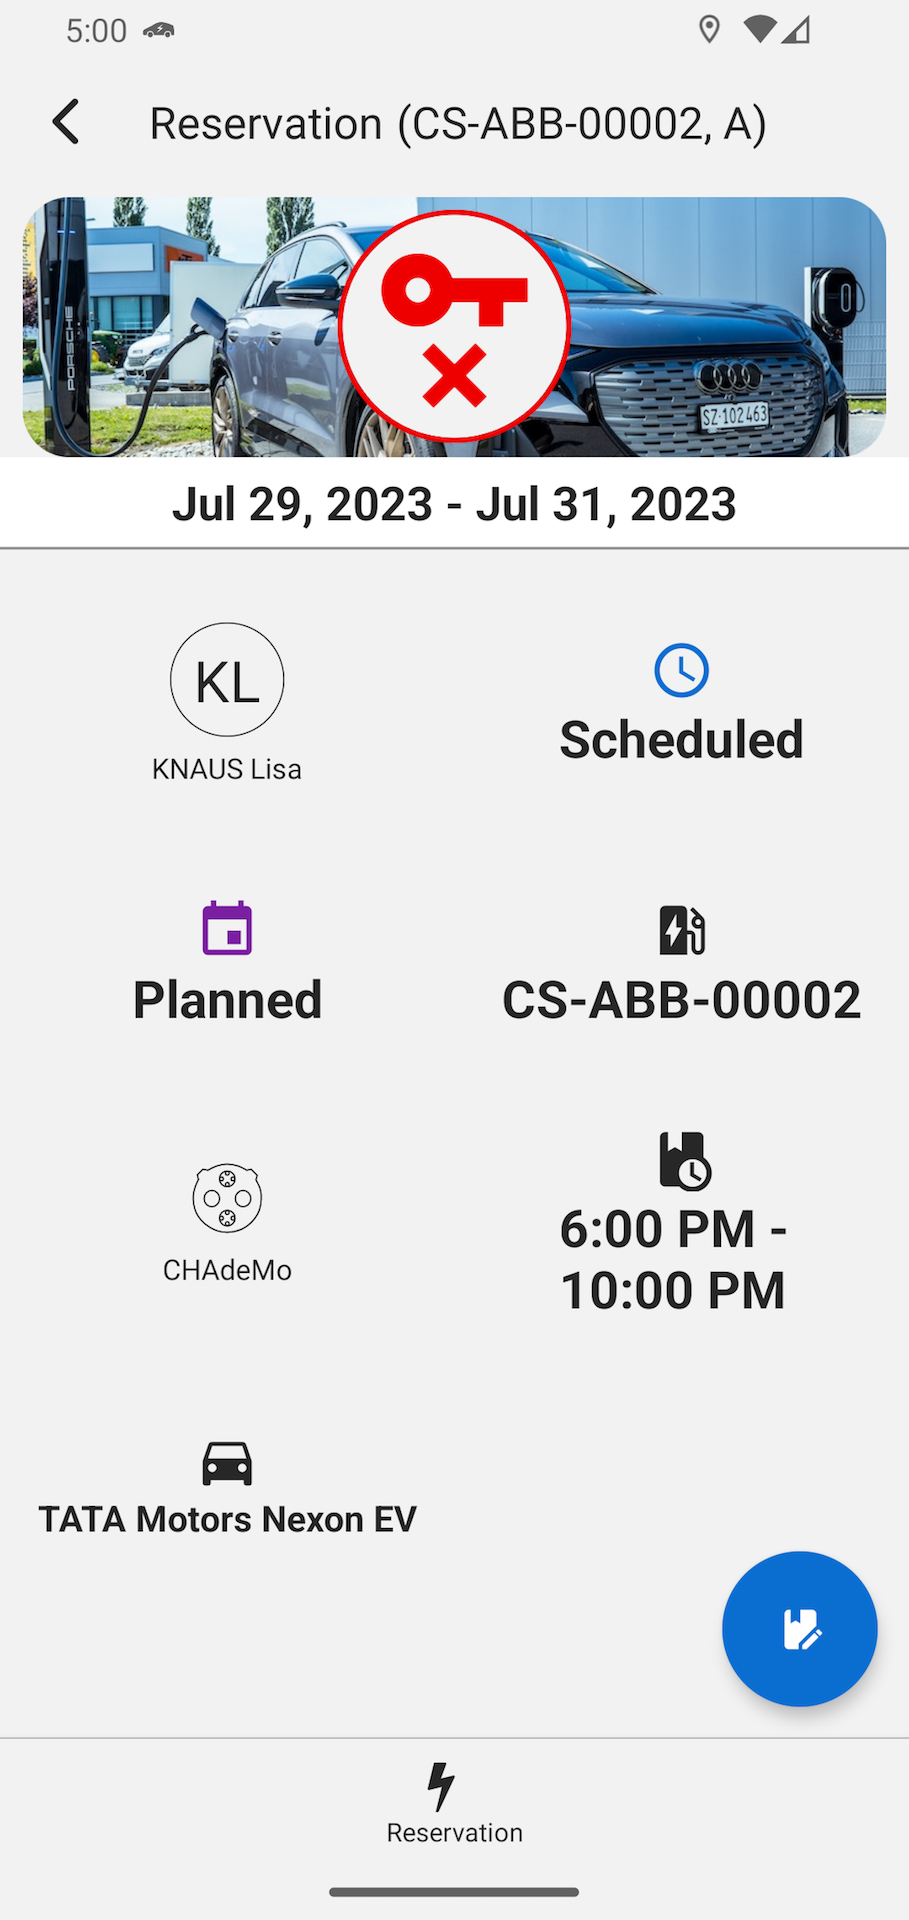
\includegraphics[width=\textwidth,height=1.6\textwidth,keepaspectratio]{resources/images/main/6_implementation/screens/cancel_reservation/mobile/Cancel_Reservation.png}
        \caption{Cancel a reservation on the mobile version from the details view of the booking.}
        \label{fig:mobile-cancel-reservation-impl}
    \end{subfigure}
    \caption{Implementation of the user interfaces of the mobile and web versions relating to the cancellation operation.}
    \label{fig:impl-cancel-reservation}
\end{figure}

\noindent To mark a booking for revocation, the related functionality could be executed using the \acrshort{rest} methodology on behalf of the following endpoint in combination with the matching \acrshort{id} as a path parameter in the \acrshort{url}.

\begingroup
\setlength{\tabcolsep}{10pt} % Default value: 6pt
\renewcommand{\arraystretch}{1.5} % Default value: 1
\begin{table}[h]
\centering
\caption{Provided \acrshort{rest} endpoints.}
    \begin{tabular}{l|c}
    Resource Identifier & HTTP Method \\ \hline
    \texttt{/reservations/\{id\}/cancel} & \texttt{PUT}
    \end{tabular}
\label{tab:cancel-reservation-rest}
\end{table}
\endgroup

\newpage

\subsubsection{Delete Reservation}
\label{ch:Implementation:sec:Reservation System:ssec:Management Capabilities:sssec:Delete Reservation}

Extending the \textbf{Cancel Reservation} functionality, \textbf{Delete Reservation} not only cancels the reservations that are currently ongoing within the system or the \acrshortpl{cs}, it also removes them from the database entirely.
As depicted in Figure \ref{fig:delete-reservation-seqflow}, when a deletion request is received from the user at the \texttt{ReservationRouter}, the \texttt{ReservationValidatorRest} validates it again and returns the process execution to the \texttt{ReservationService}. The latter continues the deletion process, once the data entered is correctly validated.
With respect to the attached \acrshort{id}, that denotes the booking the user intends to delete, the \texttt{ReservationStorage} retrieves the entity from the database and thus verifies its existence this way.
In addition to verifying the existence of the record, the current booking status is assessed to initiate additional measures for managing ongoing reservations.
This includes preventing the deletion of bookings in progress without notice, for example. To manage ongoing appointments, the system contacts the relevant stations by using the \texttt{contactChargingStation} method to release the respective \acrshortpl{cs} and connectors.
Due to the lack of a specific delete operation in the \acrshort{ocpp} standard, the deletion encapsulates the cancellation operation for a standardized communication with the \acrshort{cs}. 
As the station does not possess the ability to store history, the cancellation could be described as equivalent to a deletion at the charging infrastructure level.
After resolving the dependencies of the booking with the infrastructure, the \texttt{ReservationStorage} ultimately deletes the record in the database.

\newpage

\begin{figure}[h]
    \centering
    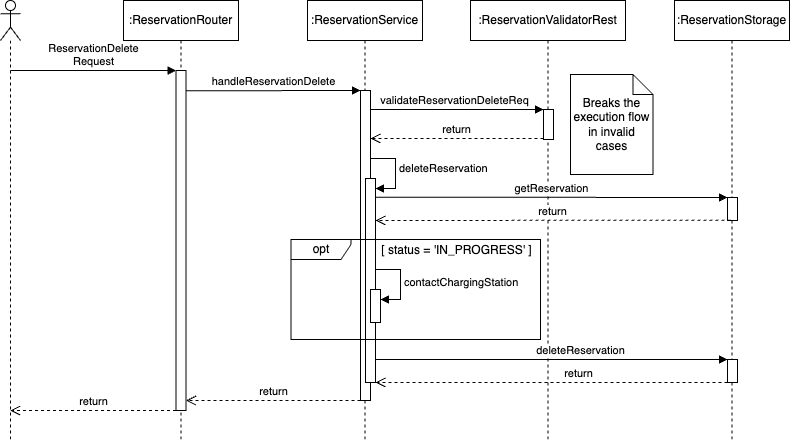
\includegraphics[scale=0.4]{resources/images/main/6_implementation/processes/ReservationDelete.png}
    \caption{Component interaction when deleting a reservation record considering the design drafts.}
    \label{fig:delete-reservation-seqflow}
\end{figure}

\noindent As well as the referred counterpart, the delete operation, is also designed in the form of a single button. It is included within every screen showing a particular booking, enabling the user to delete at least one entity inside the system.
In terms of a larger \acrshort{gui} for interaction, the browser app allows the user to delete multiple reservations at once, as indicated by the provided \acrshort{rest} endpoints in the Table \ref{tab:delete-reservation-rest}.
With reference to further development for the mobile versions, it may be feasible to implement a multi--select interface to enable the inclusion of multiple list entries within a single delete request.

\begin{figure}[h]
    \centering
     \begin{subfigure}[c]{0.6\textwidth}
         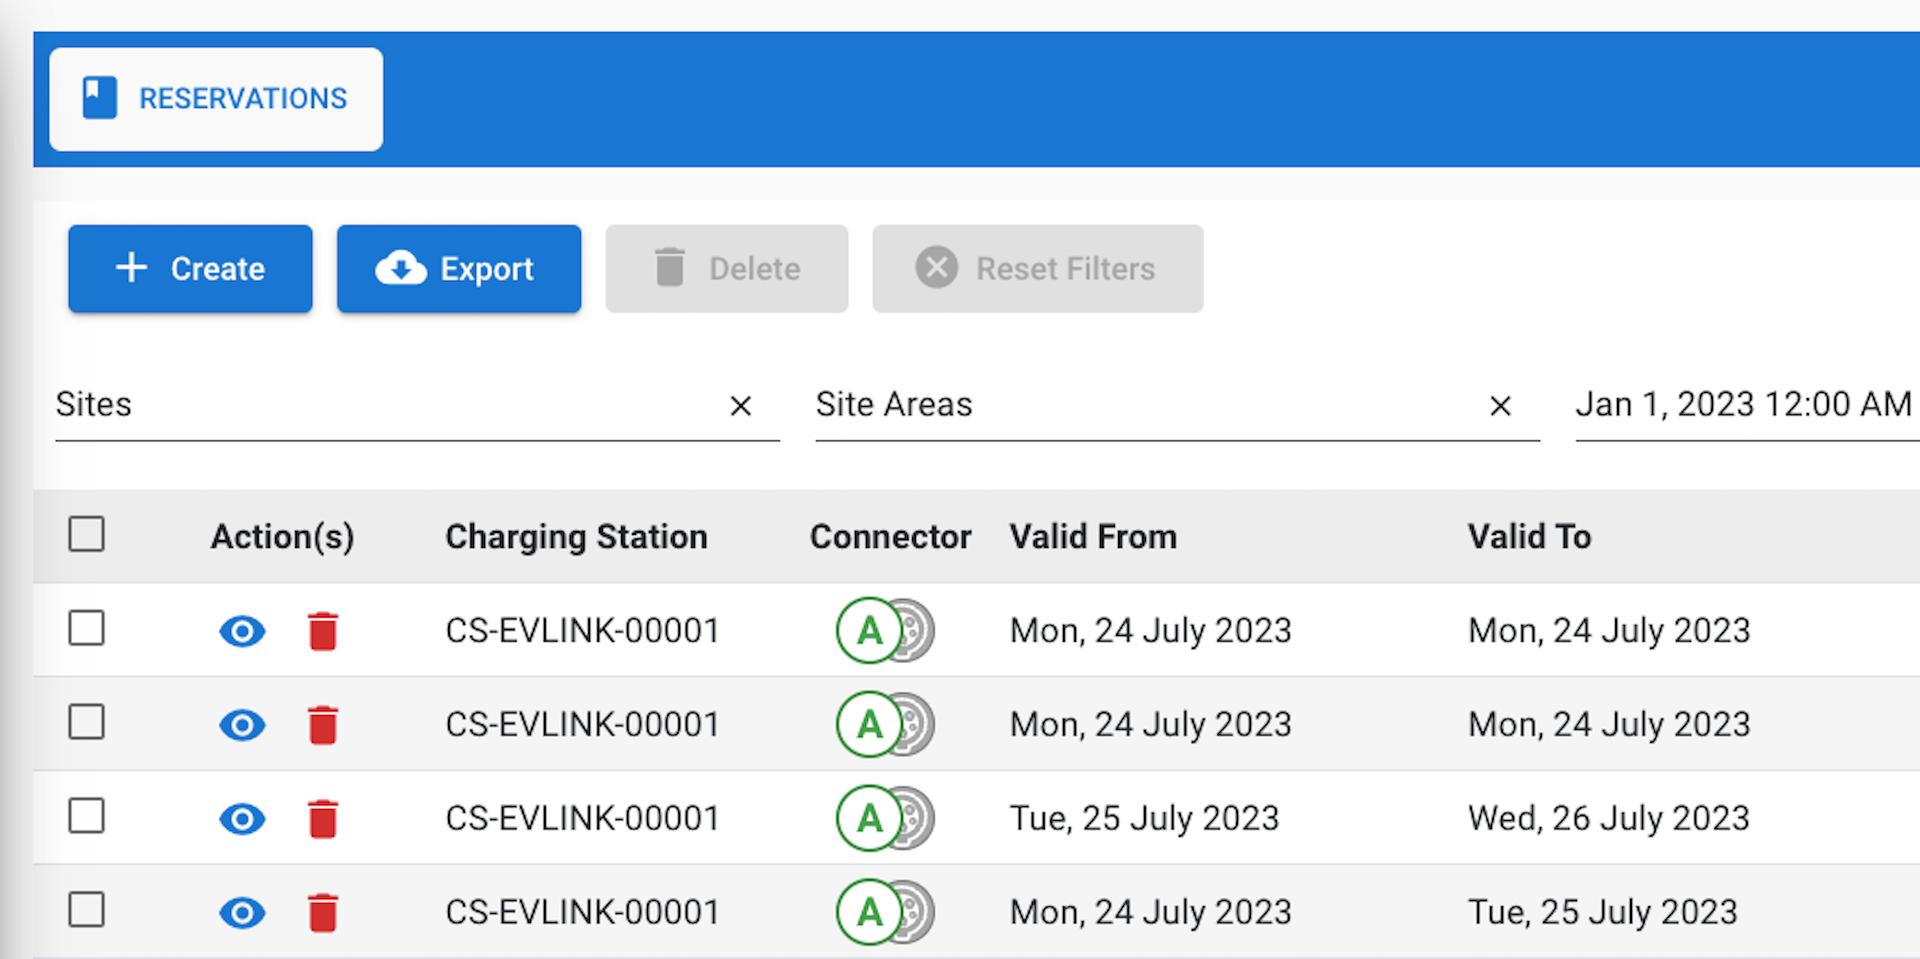
\includegraphics[width=\textwidth]{resources/images/main/6_implementation/screens/delete_reservation/web/Delete_Reservation.png}
         \captionsetup{skip=58pt}
         \caption{Delete a reservation in the browser.}
         \label{fig:web-delete-reservation-impl}
    \end{subfigure}
     \hfill
     \begin{subfigure}[c]{0.3\textwidth}
        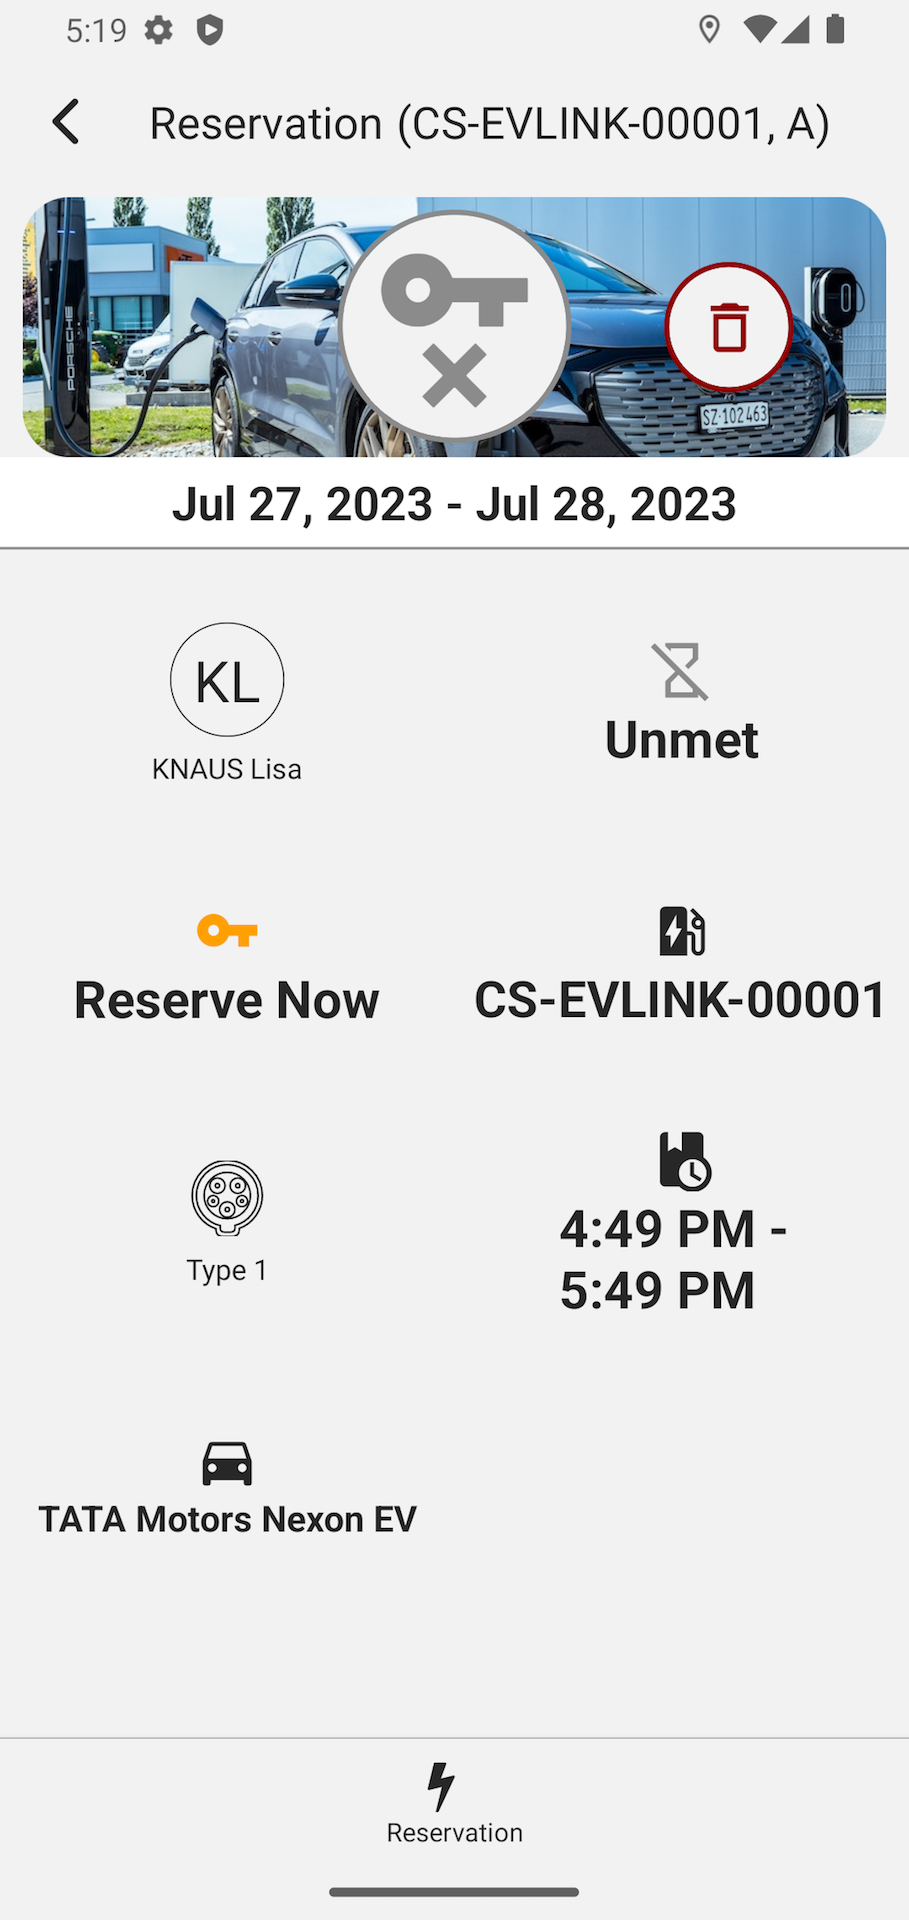
\includegraphics[width=\textwidth,height=1.5\textwidth,keepaspectratio]{resources/images/main/6_implementation/screens/delete_reservation/mobile/Delete_Reservation.png}
         \caption{Delete a reservation on the hand--held device.}
         \label{fig:mobile-delete-reservation-impl}
    \end{subfigure}
    \caption{Implementation of the user interfaces of the mobile and web application relating to the deletion of reservations using the \faIcon[solid]{trash} icon.}
    \label{fig:impl-delete-reservation}
\end{figure}

\noindent To allow both atomic and batch deletion of entities, the \acrshort{rest} methodology recommends introducing the endpoints listed in Table \ref{tab:delete-reservation-rest}. 
For distinguishing between both operations, in order to delete a single object, the user must reference it by its \acrshort{id}. 
In the case of deleting multiple entries, the user has to submit multiple entries, omitting the \acrshort{id} path parameter.

\begingroup
\setlength{\tabcolsep}{10pt} % Default value: 6pt
\renewcommand{\arraystretch}{1.5} % Default value: 1
\begin{table}[h]
\centering
\caption{\acrshort{rest} endpoints for deletion purposes.}
    \begin{tabular}{l|c}
    Resource Identifier & HTTP Method \\ \hline
    \texttt{/reservations/} & \texttt{DELETE} \\
    \texttt{/reservations/\{id\}/} & \texttt{DELETE}
    \end{tabular}
\label{tab:delete-reservation-rest}
\end{table}
\endgroup

\newpage

\subsubsection{Enable Reservations}
\label{ch:Implementation:sec:Reservation System:ssec:Management Capabilities:sssec:Enable Reservations}

Representing the final predefined management capability established during the preceding design phase, the \textbf{Enable Reservations} function enables the system administrator to activate the extension developed in this work.
This feature is part of the \texttt{Tenant Component} modules, which stand for different feature sets, the tenants can be enabled for.  
Due to the varying requirements and challenges faced by each organization, as identified by their dedicated tenant, the range of usable functionalities differs significantly. Which only requires subsets of the system's feature sets to be enabled simultaneously.
However, certain dependencies exist between the various components, which necessitate activating specific ones, in order to enable the usability as a whole. The reason for this is that each module determines the amount of data and information available to the tenant, therefore, activating a certain group of components is logical.
For example, the tenant component \texttt{Reservation} depends on the corresponding \texttt{Organization} component to get access to the \acrshortpl{cs} on the different sites of the organization and the relevant users. Otherwise, the system denies to enable this component on itself.
Components such as the \texttt{Car} component may be activated upon request, to offer a wider range of features to the particular component. In the case of the \texttt{Reservation} component, this enables the integration of cars into the reservation.
The example configuration within the administration area of the web frontend for enabling components is displayed in the following Figure \ref{fig:enable-reservation-impl}.

\begin{figure}[h]
    \centering
    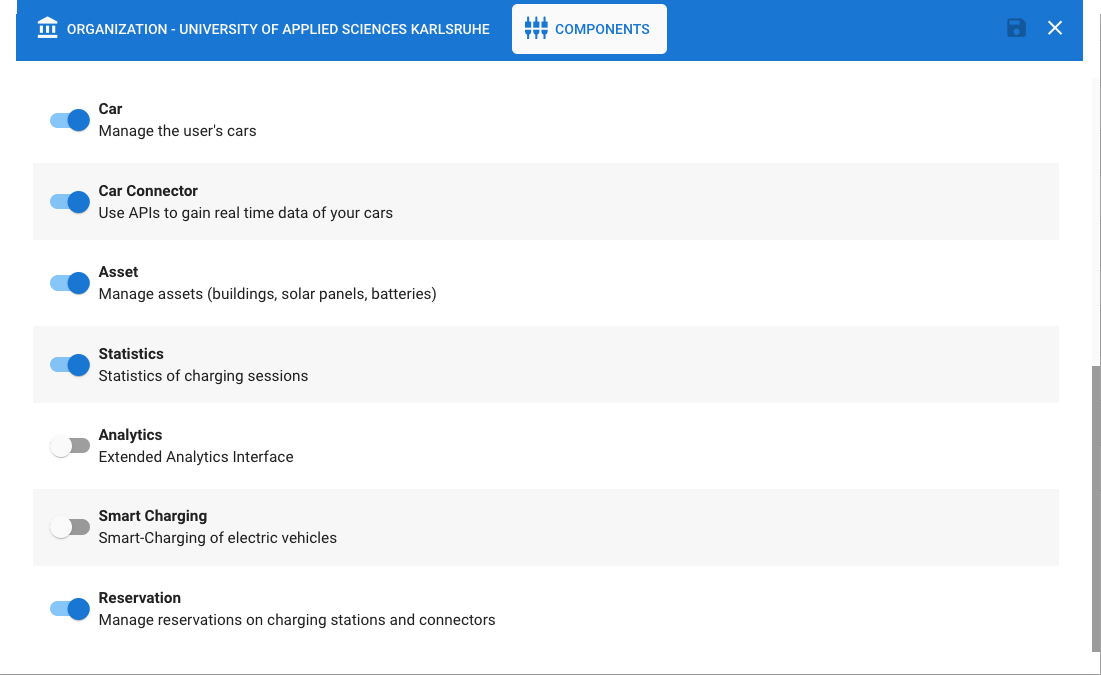
\includegraphics[scale=0.3]{resources/images/main/6_implementation/screens/enable_reservations/Reservation_Module.png}
    \caption{Implementation of the user interface for enabling the reservation module.}
    \label{fig:enable-reservation-impl}
\end{figure}

\noindent If the \texttt{Reservation} component is not active, the adjusted solution provides solely the basic \acrshort{ocpp} reservation feature set, using the standard \textit{ReserveNow} and \textit{Cancel Reservation} operations \cite{noauthor_ocpp_nodate}. 
This does not include the extension of recurring and reservations in advance, as discussed in Section \ref{ch:Implementation:sec:System Prerequisites}.

\subsection{Scheduling Capabilities}
\label{ch:Implementation:sec:Reservation System:ssec:Scheduling Capabilities}

Complementing the management capabilities covered in the previous subsection \ref{ch:Implementation:sec:Reservation System:ssec:Management Capabilities}, the ability to schedule and process pre--configured tasks automatically without any interaction is a key aspect of developing a system that manages distributed infrastructure facilities. 
To maximize automation, the proposed scheduling capabilities comprise a set of batch processing jobs, that are intended to run sequentially and can be enabled on demand within the \acrshort{json} configuration file \texttt{src/assets/config.json} included with the project. 
In addition to task activation and ensuring the specified sequential order, this file also allows for specifying the execution intervals in the form of \texttt{*/1 * * * *}, employed as the syntax for Cron jobs in the \textit{UNIX} world, to schedule job processing at specific times.
For the execution to behave as expected, the reservation component module introduced in \ref{ch:Implementation:sec:Reservation System:ssec:Management Capabilities:sssec:Enable Reservations} must be enabled. Otherwise, regardless of the activation, these tasks are not running.
The pivotal function for handling these tasks is represented by the \texttt{TenantSchedulerTask} already mentioned as one of the key components for the working system in \ref{ch:Implementation:sec:Reservation System:ssec:Architectural Views:sssec:Components}.
As the top--level entity overseeing all available tasks for execution, it executes the activated ones at their designated time intervals on the server.
The recommended sequence for executing the subsequent jobs to ensure correct operation is defined as follows within the context of this work:
\begin{description}
    \item[]{\makebox[5.5cm][l]{\textbf{Schedule Reservation:}} \texttt{*/5 * * * *} \quad \textit{'Executed every five minutes.'}}
    \item[]{\makebox[5.5cm][l]{\textbf{Expire Reservation:}} \texttt{*/4 * * * *} \quad \textit{'Executed every four minutes.'}}
    \item[]{\makebox[5.5cm][l]{\textbf{Free Reserved Connectors:}} \texttt{*/1 * * * *} \quad \textit{'Executed on a minute basis.'}}
\end{description}

\subsubsection{Schedule Reservation}
\label{ch:Implementation:sec:Reservation System:ssec:Scheduling Capabilities:sssec:Schedule Reservation}

Due to the fact that the user can create reservations in the future, the corresponding \acrshortpl{cs} and the system itself must be notified when the reserved time period arrives. \\
To do this, the \textbf{Schedule Reservation} task shown in Figure \ref{fig:schedule-reservation-seqflow}, implemented as \\ \texttt{SynchronizeReservationTask}, loads all reservations with status \texttt{SCHEDULED} for the next 15 minutes from the database.
Also, to enable recurrent events, this comprises bookings with the status \texttt{IN\_PROGRESS} as well. 
In the further processing of the combined booking types, the \texttt{synchronizeWithChargingStation} method checks for currently running charging sessions on the respective stations and connectors. If these sessions are not assigned to the \acrshort{rfid} tag, that belongs to the reservation, the method stops them immediately.
To address this, the \texttt{ChargingStationClient} is used, which is a product of the \texttt{ChargingStationClientFactory}, that controls instantiation using factory methods, to communicate directly with the \acrshort{cs}.
Otherwise, the reservation is made directly on the \acrshort{cs} and if it has a \texttt{SCHEDULED} status, it is adjusted accordingly. A notification is then sent to the user, via the \texttt{NotificationHelper}, to inform that a booked charging session is forthcoming.
Besides saving the updated record, its \acrshort{id} is assigned to the associating connector on the \acrshort{cs} in the database, using the \texttt{updateConnectorWithReservation} method.

\begin{figure}[h]
    \centering
    \includegraphics[scale=0.4]{resources/images/main/6_implementation/processes/scheduler/SynchronizeReservation.png}
    \caption{Interaction between relevant components to synchronize the reservations with the associated \acrshortpl{cs} taking into account the underlying process design.}
    \label{fig:schedule-reservation-seqflow}
\end{figure}

\newpage

\subsubsection{Expire Reservation}
\label{ch:Implementation:sec:Reservation System:ssec:Scheduling Capabilities:sssec:Expire Reservation}

After having automatically synchronized the reservations with the corresponding \acrshortpl{cs}, a routine to clean up the expired ones and to fulfill certain aspects of the householding tasks is implemented as \texttt{CheckReservationStatusTask}.
Designed as a counter piece to \textbf{Schedule Reservation}, this job deals with entities reaching their expiration date, as demonstrated in Figure \ref{fig:expire-reservation-seqflow}.
To identify the concerned bookings, it loads each record with a status of \texttt{IN\_PROGRESS} or \texttt{SCHEDULED} and an expiry date that is overdue by the current time and date.
If any record is found, the task then iterates through the list of reservations and removes the reservation information from the associated connector, using \texttt{resetConnectorReservation}. 
As a complement to the \texttt{updateConnectorWithReservation} function mentioned in the previous process, this method is used when an arrangement still blocks a connector after it is successfully cancelled or deletion. This is often due to the system disconnecting from the \acrshort{cs} during the latter stages of the process.
Considering this case, it is utilized to invalidate expired bookings, change their status to \texttt{EXPIRED} in the database, and notify the involved profile with the \texttt{NotificationHelper}.

\begin{figure}[h]
    \centering
    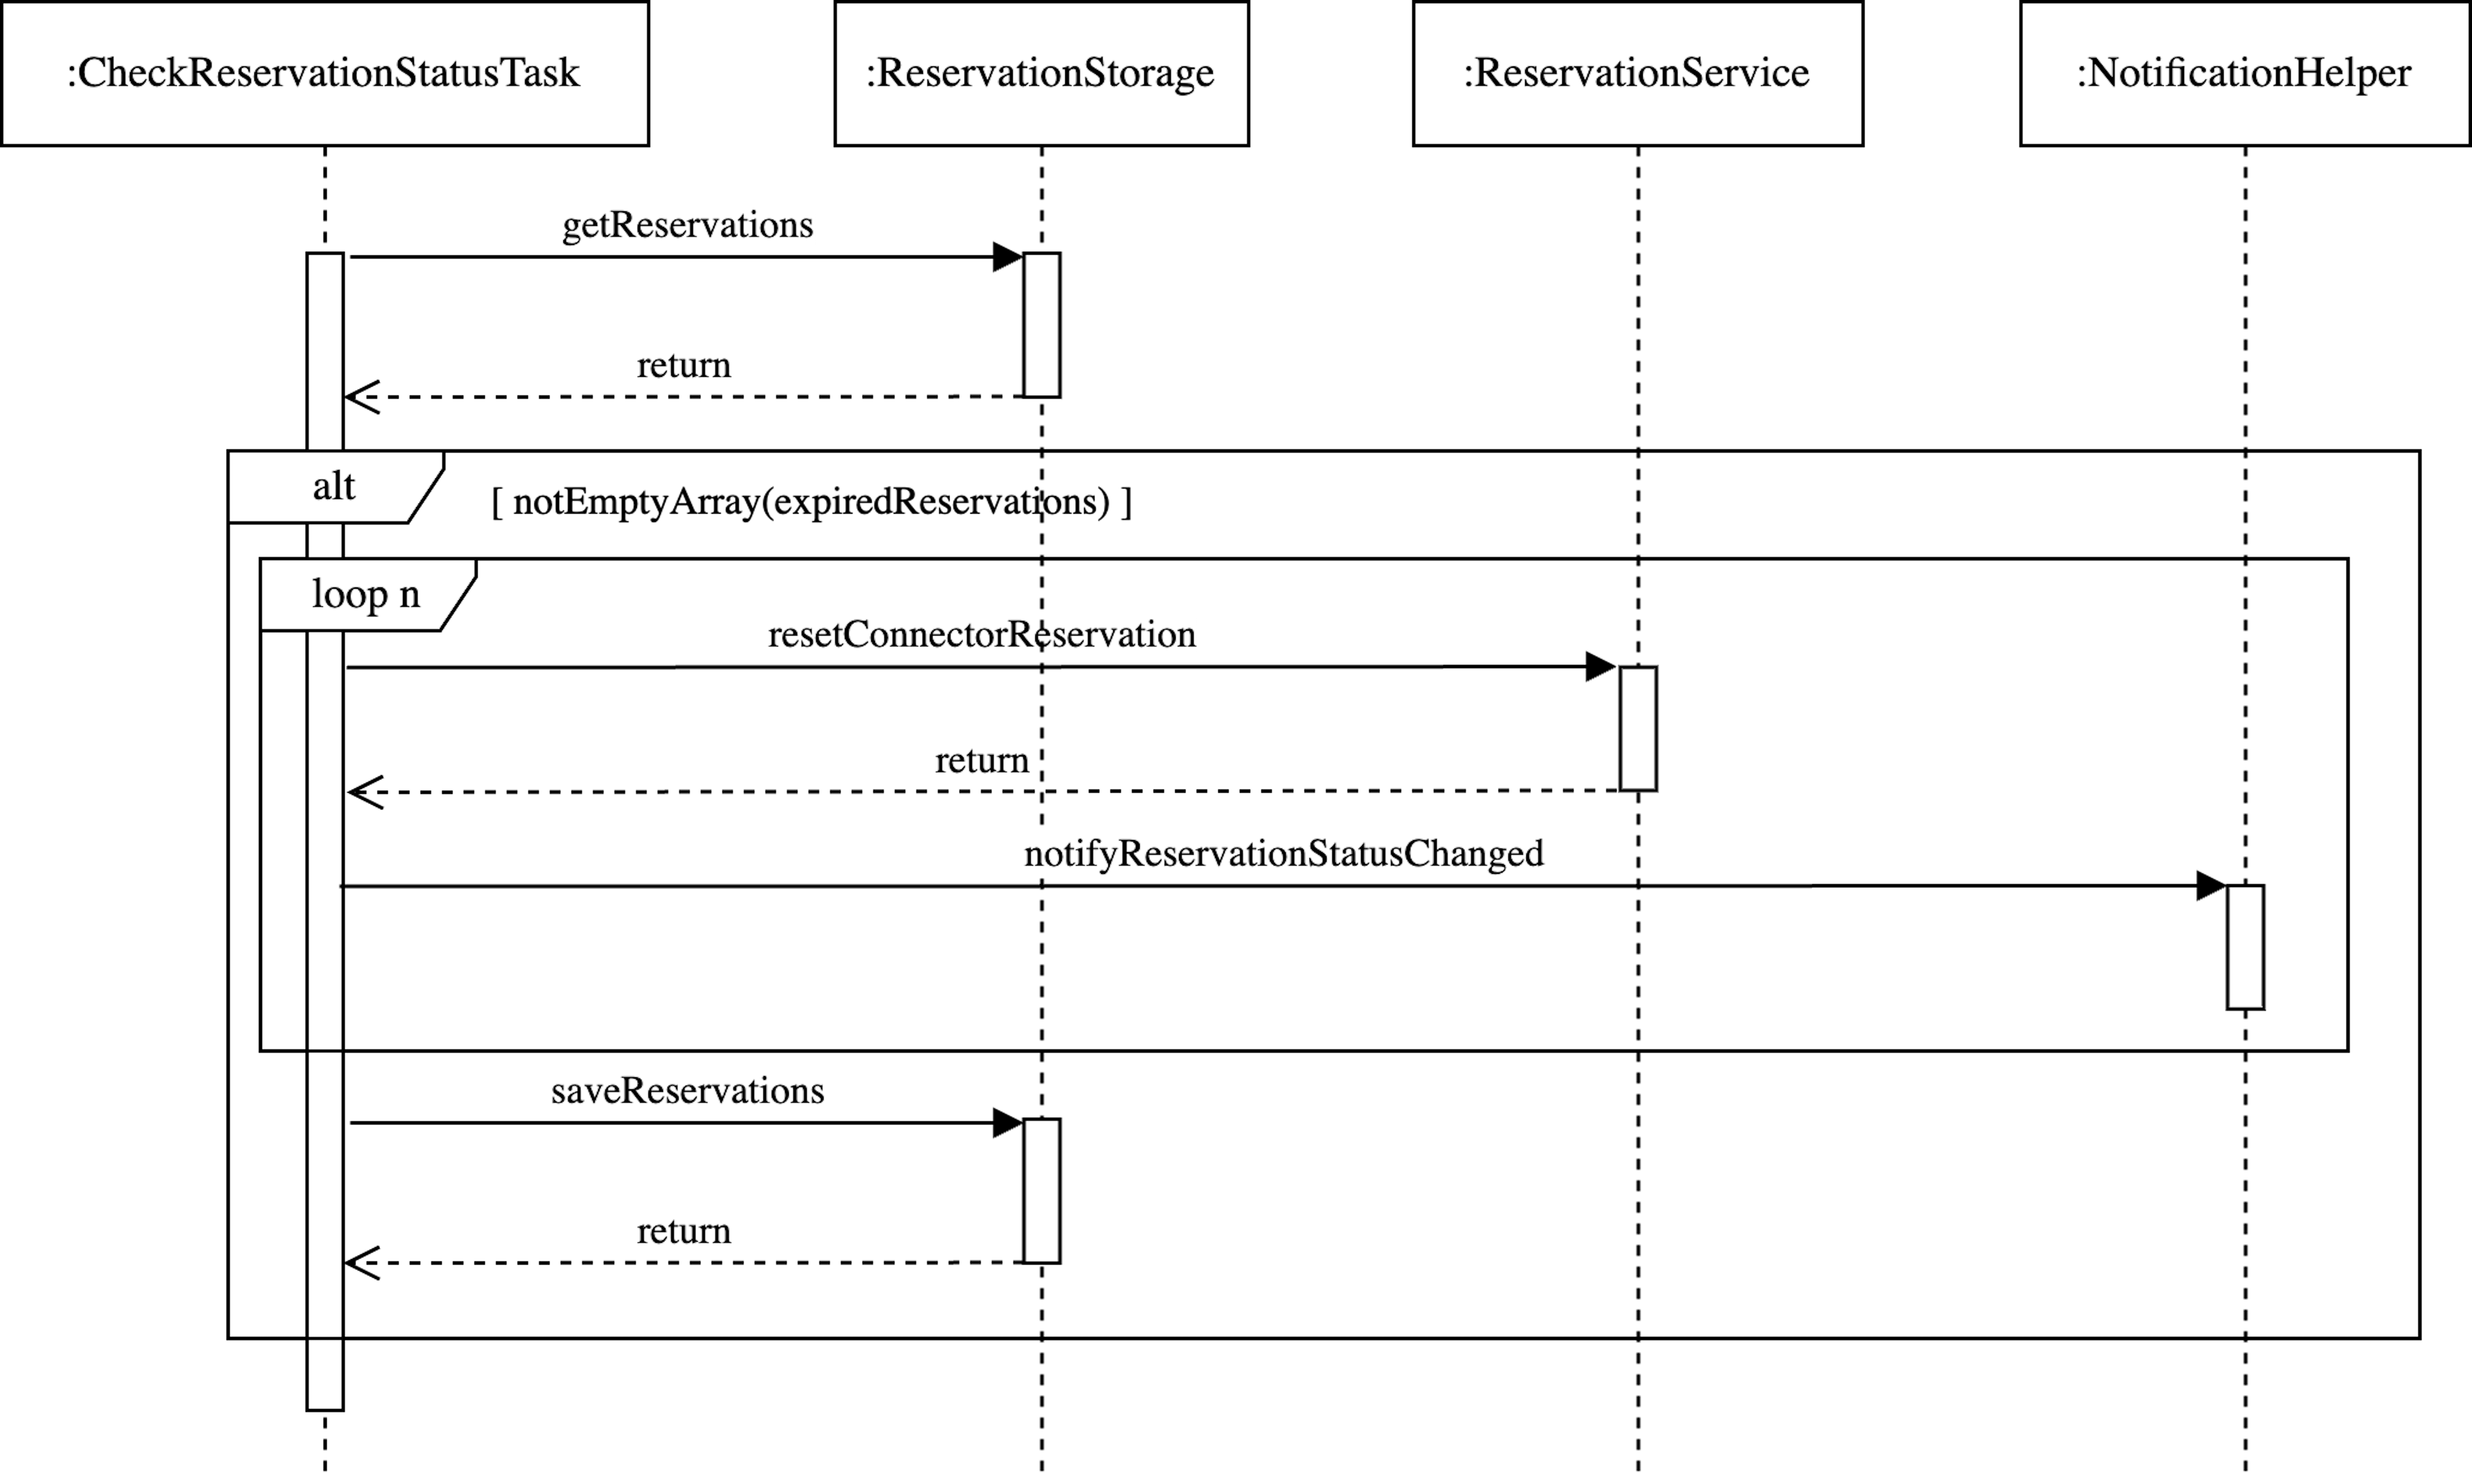
\includegraphics[scale=0.5]{resources/images/main/6_implementation/processes/scheduler/UpdateExpiredReservations.png}
    \caption{Sequential flow of the components interacting with each other, to invalidate expired bookings using the considered process templates.}
    \label{fig:expire-reservation-seqflow}
\end{figure}

\newpage

\subsubsection{Free Reserved Connectors}
\label{ch:Implementation:sec:Reservation System:ssec:Scheduling Capabilities:sssec:Free Reserved Connectors}

While the \textbf{Expire Reservation} function looks after the expiry as a natural element of the booking life cycle, the \textbf{Free Reserved Connectors} task has a more regulative purpose.
Taking the position of an imaginary steward, it monitors all ongoing engagements on the \acrshortpl{cs} and identifies the ones, where the user has not arrived after a certain period of time after the supposed arrival time.
Following the \acrshort{ocpp} standard, the arrangement lasts until the expiry time is reached. As the expiration time is undefined, it could be several hours later and block the station during this time. 
To mitigate this issue in the handling of reservations, the proposal provides a background task, implemented in \texttt{CancelUnmetReservationsTask} and described in Figure \ref{fig:free-connector-seqflow}.
As a result of this custom implementation, it is possible to handle unfulfilled reservations, due to a certain threshold defined by the constant \texttt{THRESHOLD}, which is set to \textbf{15} minutes in the context of this work.
Every booking with an arrival time exceeding this threshold is identified by the \texttt{ReservationStorage}. If the associated connector is still in the \texttt{RESERVED} state, the blockage is cancelled to free the reserved charging unit.
Otherwise, the next one is evaluated by using these constraints.
After setting all identified entries meeting these criteria to the \texttt{UNMET} status and saving them again, the relevant individuals are informed of their undesired conduct.

\begin{figure}[h]
    \centering
    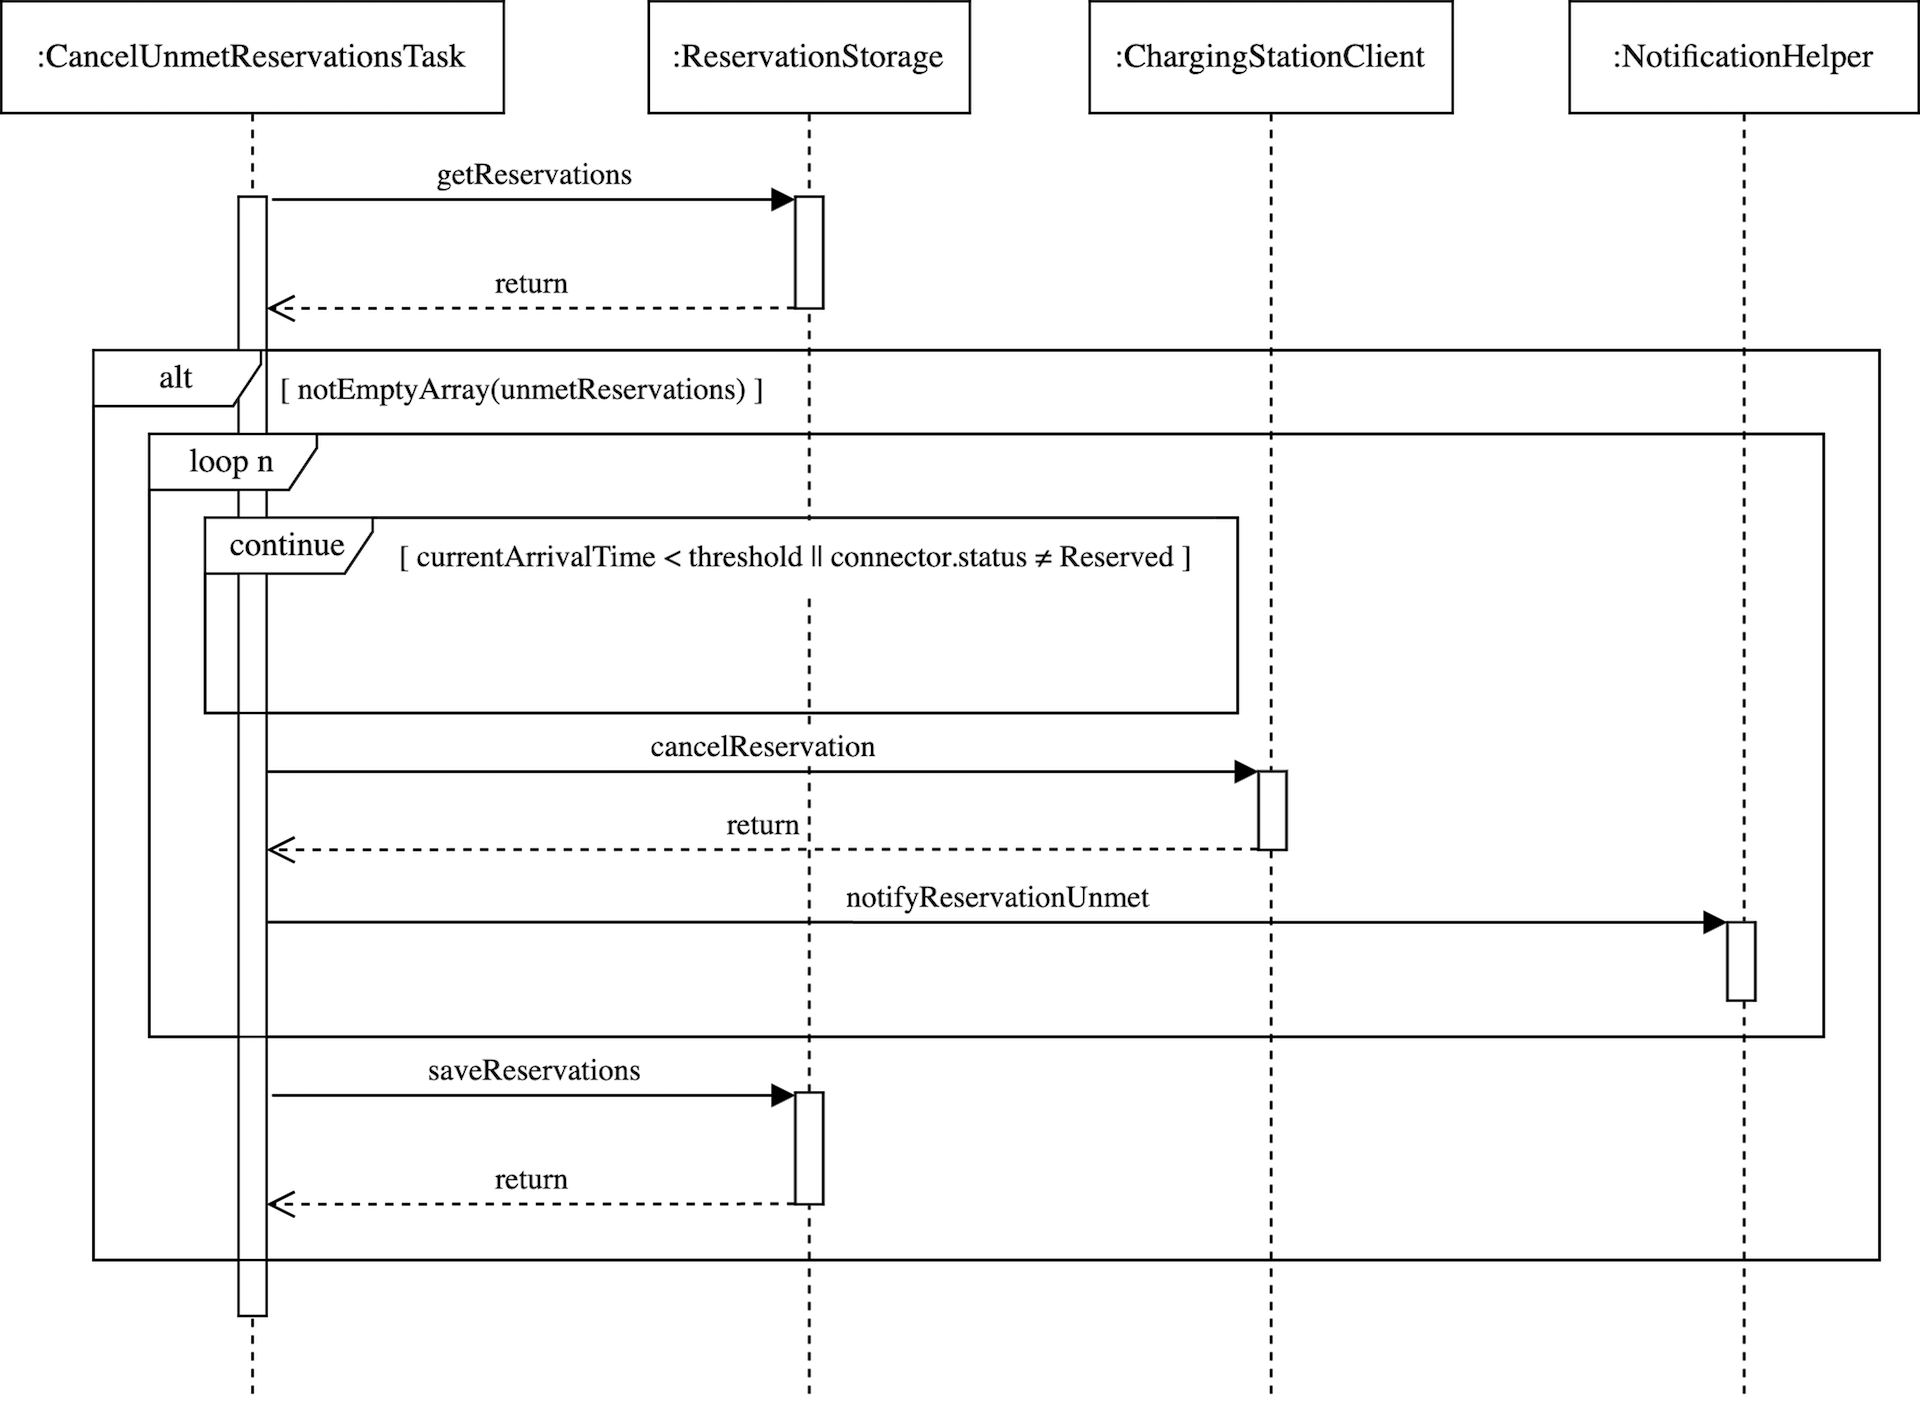
\includegraphics[scale=0.5]{resources/images/main/6_implementation/processes/scheduler/CancelUnmetReservation.png}
    \caption{Required component interactions for removing unmet appointments on the respective \acrshortpl{cs} in order to implement the underlying design proposals.}
    \label{fig:free-connector-seqflow}
\end{figure}

\newpage

\subsection{Notification Capabilities}
\label{ch:Implementation:sec:Reservation System:ssec:Notification Capabilities}

With regard to the notification types, introduced to cover different scenarios in the application and arrangement lifetime, this subsection provides a brief overview of which notification types are actually used within the implemented features.
This may serve as a reference point for future implementations and as a possibility to evaluate new scenarios not covered by this implementation.
Implied by the listing of involved packages in subsubsection \ref{ch:Implementation:sec:Reservation System:ssec:Architectural Views:sssec:Packages}, particularly by viewing the \texttt{notification} package, the system can send notifications in various forms.
Alongside using the \acrshort{smtp} protocol \cite{klensin_simple_2008} primarily targeting adopters of the browser app with assumed easier access to their mail clients, for the mobile apps the service utilizes Google's Firebase \cite{noauthor_firebase_nodate} \acrshort{paas} and \acrshort{iaas} offer to publish information via push notifications.
During the development phase as part of the extension for the mobile component of the project, this work has identified missing functionalities related to background notifications, when the application is closed or not opened. To address this specific feature gap, adjustments to the appropriate logic and the \texttt{notifee/react-native} package from Notifee \cite{noauthor_notifee_nodate} are added.
Seizing the suggestions presented in the \textbf{Scheduling Capabilities} subsection of the design chapter \ref{ch:Design:sec:Reservation System:ssec:Scheduling Capabilities}, the notification types such as \texttt{ReservationStatusChanged}, \texttt{ReservationUpcoming}, \texttt{ReservationCreated}, \texttt{ReservationCancelled} and \texttt{ReservationUnmet} are utilized in the current tasks to convey crucial information about the processed entities to the end users and facilitate the information flow.
This should ensure that the \acrshort{evu} can make informed decisions based on up--to--date information provided by the system.
In the case of the \texttt{ChargingStationBlocked} notification, no suitable location could be identified. An integration within the \textbf{Schedule Reservation} process would lead to a simultaneous notification of the user blocking the \acrshort{cs}, as well as the user of the reservation. 
Possibly resulting in the parallel switching of drivers to a new station and the situation that this notification was intended to prevent. \\
\noindent In terms of the support for multiple languages both the notifications and the labels of the \acrshort{gui} elements, which normally adapt to the language set in the user's profile, are only translated into English and German.
Other language options, including Spanish, French, and Italian, are not part of this approach and further work needs to be done to allow these languages to be used properly.

\subsection{Additional Capabilities}
\label{ch:Implementation:sec:Reservation System:ssec:Additional Capabilities}

During development, more ways to enhance the reservation approach with extended features beyond the defined use cases could be identified.
These capabilities, since they have no direct use affecting the basic functionality in interaction with the system, are listed as \textbf{Additional Capabilities} and are mentioned here as part of an informative section, to possibly be considered as useful for other scenarios, that may arise during other studies in this area.

\subsubsection{Export Reservation}
\label{ch:Implementation:sec:Reservation System:ssec:Additional Capabilities:sssec:Export Reservation}

By examining the backend service features and frontends' specific functions, the potential to export certain entities of the system in the form of generated \acrshort{csv} reports stands out.
Despite the fact that it was not considered during the design of the system, the author of the work assumes that this feature could be useful for the end users of the platform in the context of data recovery and analysis purposes.
Representing a very basic functionality, which only requires extracting all specified entries from the database and transforming them into a \acrshort{csv} compliant format, no additional process or sequence flow is elaborated.
Implemented as a button on the reservation overview interface within the web \acrshort{gui}, the \textbf{Export Reservation} functionality loads each booking the user has access to from the database and writes the entries into a \acrshort{csv} compliant file that can be downloaded via the browser.
If the database crashes or there is a risk of unwanted data loss, these files could be the basis for populating new instances of the system or recreating a clean application state.

\noindent As a dedicated endpoint on the web server, this functionality is provided, using the \acrshort{rest} methodology and the relevant resources as part of the service portfolio and is presented in the subsequent Table \ref{tab:export-reservation-rest}.

\begingroup
\setlength{\tabcolsep}{10pt} % Default value: 6pt
\renewcommand{\arraystretch}{1.5} % Default value: 1
\begin{table}[h]
\centering
\caption{Endpoint for exporting the booking entries inside the database.}
    \begin{tabular}{l|c}
    Resource Identifier & HTTP Method \\ \hline
    \texttt{/reservations/action/export} & \texttt{GET}
    \end{tabular}
\label{tab:export-reservation-rest}
\end{table}
\endgroup

\subsubsection{Reservable Charging Stations}
\label{ch:Implementation:sec:Reservation System:ssec:Additional Capabilities:sssec:Reservable Charging Stations}

Due to the assumption, that the individuals create their reservations directly by selecting the \acrshortpl{cs} from the map view, considered as the entry point of the mobile application, or by using the various filter options within the web app, a pre--filtering mechanism to narrow down the options for available stations during a specific time in the future was not included in the design.
However, the proposed solution provides a method for making bookings without pre--selecting the \acrshort{cs}, which leads to the requirement of choosing a suitable station, while setting the reservation constraints. To promote a more convenient recommendation mechanism, the creation process should be supported by minimizing the number of stations presented, that are not otherwise occupied at the given time.
Taking this into account, the initial concept of the underlying logic resembles a simple intersection, similar to the one shown in Figure \ref{fig:reservable-cs}. In this way, the appropriate subset of connectors available for reservation could be easily identified.
Hence, the code loads all the entries for the specified period and all the \acrshortpl{evse} registered in the system, in order to perform an intersection of the two sets and select only the stations inside the \textbf{blue area}, as shown in the diagram below. These stations comprise the subset of options to be offered by the input fields.
If other \acrshortpl{evu} create reservations during this process, that would affect the offered selection, the service should detect any resulting overlaps and handle them appropriately as usual.

\begin{figure}[h]
    \centering
    \begin{tikzpicture}[
        set/.style = { circle, minimum size=4cm}]
        \node[set,fill=blueprimary,label={45:$Charging\ Stations$}] (cs) at (0:3) {};
        \node[set,fill=white,label={135:$Reservations$}] (r) at (0,0) {};
        \draw (0,0) circle(2.0cm);
        \draw (3,0) circle(2.0cm);
        \node[right,white,xshift=-0.2cm] at (cs.center){$Reservable$};
    \end{tikzpicture}
    \caption{Isolation of reservable \acrshortpl{cs} utilizing an intersection with already reserved ones.}
    \label{fig:reservable-cs}
\end{figure}

\noindent As the client applications must pre--populate input fields in the appropriate \acrshort{gui} windows, this supporting functionality is triggered by the respective endpoints listed in the Table \ref{tab:reservable-cs-rest}. To implement this feature, the selected design approach requires expanding the relevant \texttt{charging-station} \acrshort{rest} resource, which is managed by the \texttt{ChargingStationService} and the upstream \texttt{ChargingStationRouter}.

\begingroup
\setlength{\tabcolsep}{10pt} % Default value: 6pt
\renewcommand{\arraystretch}{1.5} % Default value: 1
\begin{table}[h]
\centering
\caption{Added \acrshort{rest} endpoint to provide the subset of reservable \acrshortpl{cs}.}
    \begin{tabular}{l|c}
    Resource Identifier & HTTP Method \\ \hline
    \texttt{/charging-stations/reservation/availability} & \texttt{GET}
    \end{tabular}
\label{tab:reservable-cs-rest}
\end{table}
\endgroup

\subsubsection{Reservation Retrieval}
\label{ch:Implementation:sec:Reservation System:ssec:Additional Capabilities:sssec:Reservation Retrieval}

Besides the aforementioned feature sets and their related endpoints, a web service following the \acrshort{rest} architectural model requires additional interfaces, e.g. for information retrieval.
Consequently, according to this approach, endpoints must be supplied for so--called \texttt{READ} operations. The function's connotation implies, that these endpoints are accessible for requesting data when calling the corresponding \acrshort{url}.
Following the naming convention of the \acrshort{rest} method, the resource for collecting reservations is declared, as its plural form of the handled entity name in lowercase. Given the proposed solution and the reservation as the underlying entity, the resource provided by this system is called \texttt{reservations}.
Resulting in the interfaces listed in Table \ref{tab:read-reservations-rest} and accessible through the reservation \acrshort{api}, mainly employed for providing clients access to the internal system information.

\begingroup
\setlength{\tabcolsep}{10pt} % Default value: 6pt
\renewcommand{\arraystretch}{1.5} % Default value: 1
\begin{table}[h]
\centering
\caption{\acrshort{rest} endpoints for performing \texttt{READ} operations retrieving reservation entities.}
    \begin{tabular}{l|c|m{5cm}}
    Resource Identifier & HTTP Method & Functionality \\ \hline
    \multicolumn{3}{c}{\texttt{/reservations}} \\ \hline
    \texttt{/} & \texttt{GET} & Retrieve all reservations available \\
    \texttt{/\{id\}} & \texttt{GET} & Request for a specific reservation by its \acrshort{id} \\
    \end{tabular}
\label{tab:read-reservations-rest}
\end{table}
\endgroup

\newpage

\subsection{Role Concept}
\label{ch:Implementation:sec:Reservation System:ssec:Role Concept}

To assign the necessary functionality to each system role, as described in the chapter of requirements engineering, particularly Section \ref{ch:Requirements Engineering:sec:Role Mapping}, the capabilities required to fulfill their purpose must be considered according to the principles of least privilege, which are explained in \cite{ma_specifying_2011}.
Additionally, to supplement the mapping of feature sets to roles, the solution distinguishes between specific scopes that describe the range of information available to that particular role.
Roles assigned with the \textit{Own} scope only have access to their own data and cannot view reservations made by other profiles, for example.
That falls within the scope of the \textit{Site}, allowing the assigned role to access all data pertaining to that specific location.
With this privilege, the respective user can create, update, or cancel bookings for all users assigned to this site, for instance. An exception to this privilege set is the \textit{Admin} role, which is not limited to a dedicated site and allows the user to manage all entities, related to the entire tenant. 
Concerning the use cases from Chapter \ref{ch:Requirements Engineering} and their associated actors, the final mapping of the developed processes is presented in Table \ref{tab:role-function-mapping} as defined in the file \texttt{AuthorizationsDefinition.ts} as part of the backend project.

\begingroup
\setlength{\tabcolsep}{10pt} % Default value: 6pt
\renewcommand{\arraystretch}{1.5} % Default value: 1
\begin{table}[h]
    \centering
    \caption{Mapping of the designated reservation functionalities to the corresponding roles in the system.}
    \begin{tabular}{c|c|m{9.5cm}}
        Role & Scope & Functionality \\
        \hline
        Basic & Own & Create Reservation, Update Reservation, Cancel Reservation \\
        Admin & - & Create Reservation, Update Reservation, Cancel Reservation, Delete Reservation \\
        Site Admin & Site & Create Reservation, Update Reservation, Cancel Reservation \\
        Site Owner & Site & Create Reservation, Update Reservation, Cancel Reservation \\
        Super Admin & - & Enable Reservations \\
        Demo & Own & Create Reservation, Update Reservation, Cancel Reservation \\
    \end{tabular}
    \label{tab:role-function-mapping}
\end{table}
\endgroup

\noindent Afterwards, the assignment decisions in the context of the \textit{Delete Reservation} and \textit{Enable Reservations} actions are revisited, for a better understanding. The choice to only allow the \textit{Admin} user to perform the \textit{Delete Reservation} action is not solely based on the use case design.
This work assumes, that disruptive actions, such as entity deletion, should only be carried out when excluding system users and removing their information, which can be classified as an administrative task and solely limited to system administrators.
Concerning basic users, it is more likely that they use the cancel operation to properly revoke their reservations than to delete them completely.
In the case of the \textit{Enable Reservations} task, only the \textit{Super Admin} can access the relevant sections of the administration dashboard to configure the tenants, thus, making this role the exclusive entity for assigning this feature. 
On the other hand, this profile is unable to manage entities within the particular tenants itself, hence the need to assign it additional privileges for managing reservations is mandatory. 

\newpage

\subsection{Failure Indication}
\label{ch:Implementation:sec:Reservation System:ssec:Failure Indication}

The introduction of new features not only creates new possibilities for the interaction with the audience but also opens up a wider surface for possible unexpected circumstances, that may arise along certain scenarios. 
Most of these exceptions may occur in a way that only the system can recognize and are typically hidden from the user, who is simply experiencing the consequences, resulting from these malfunctions.
To alleviate these uncertainties, a software solution should always inform the user of its current status within the process it performs. This involves notifying the client, on behalf of the user, of any unexpected behavior that could interrupt the current operation or lead to a bad result.
Due to the nature of distributed systems, the client and the corresponding server are decoupled, and the only way the server could keep the client informed of the above scenarios is to use the \acrshort{http} status codes as part of each request to exchange information.
Apart from failures within the system itself in the form of outages or targeted attacks, the charging infrastructure and the associated \acrshortpl{cs}, should also be considered as an extra source of errors. 
To effectively identify and manage exceptions in both the backend and frontend applications, this study translated each potential exception into a status code for meaningful reservation error handling.

\newpage

\noindent The list below only reflects the current state of implementation, concerning the aforementioned range of capabilities, as well as the current state of the \acrshort{ocpp} standard, which is not meant to be complete. Potentially, additional scenarios and relevant exception--handling mechanisms need to be incorporated in the future.

\begin{multicols}{2}
\begin{description}
    \item[\texttt{600}] Reservation Already Exists
    \item[\texttt{601}] Reservation Collision
    \item[\texttt{602}] Reservation Not Supported *
    \item[\texttt{603}] Reservation Rejected *
    \item[\texttt{604}] Reservation Faulted *
\end{description}
\begin{description}
    \item[\texttt{605}] Reservation Occupied *
    \item[\texttt{606}] Reservation Unavailable *
    \item[\texttt{607}] Multiple Reserve Now
    \item[\texttt{608}] Invalid Status Transition Error
\end{description}
\end{multicols}

\noindent To distinguish the exceptions that may arise from the charging infrastructure, the respective entries in the above list are marked with the * symbol. For a detailed explanation of these particular error scenarios, please refer to the official \acrshort{ocpp} standard \cite{noauthor_ocpp_nodate}.
